\section{進一步的申述}
\label{sec:b3_ch5}

\renewcommand{\thefigure}{5-\arabic{figure}}
\setcounter{figure}{0}

\subsection*{大綱}

\begin{itemize}[leftmargin=2em]
  \item[$\ddagger$ § 5-1] \textbf{線性關聯與共線共面問題}
  \begin{itemize}[leftmargin=2em]
    \item[甲、] 三點共線
    \item[乙、] 四點共面
  \end{itemize}
  \item[$\ddagger$ § 5-2] \textbf{距離}
  \begin{itemize}[leftmargin=2em]
    \item[甲、] 點與直線
    \item[乙、] 直線與直線的距離
  \end{itemize}
  \item[* § 5-3] \textbf{座標與向量進一步的混合運用}
  \item[$\ddagger$ § 5-4] \textbf{幾個利用古典平面幾何處理的極小問題}
  \begin{itemize}[leftmargin=2em]
    \item[甲、] 光的反射
    \item[乙、] 到三定點的最小距離和
    \item[丙、] 連結三角形三邊的最短路徑
  \end{itemize}
\end{itemize}

\begin{center}
* \qquad * \qquad * \qquad * \qquad *
\end{center}

在解釋幾何與代數間的系統轉化這一層過程中，我們已介紹過向量代數（第三章），接著把笛卡兒的座標觀點引進來（第四章 § 4-1～§ 4-4）．並在第四章 § 4-5 以後開始混合運用這兩種轉化觀點——向量與座標——來處理一些幾何問題．

這一章前兩節我們要進一步發揮這兩種觀點的長處，看看這兩種系統的轉化方法，如何把幾何的問題搬到代數中去討論、推演與計算，如何把這些計算的結果又搬回幾何來．

另一方面，在一些較直觀的問題上，我們仍承認以全等三角形定理為核心的古典平面幾何的價值．從第三節\phantomsection\label{note:b3-ch5-p224-sec-ref}\footnote{【原書註記/校訂】：原書印作「從第三節所談到的一些實際的極小問題中」，但極小問題實際討論於本章第四節 § 5-4「幾個利用古典平面幾何處理的極小問題」．}所談到的一些實際的極小問題中，我們可以看出這樣的觀點仍然是值得保留且加以申述的，雖然利用（大學）微積分，這樣的極小問題也可以系統化地來解決．

原則上第三冊的討論範圍局限在“線性”部份．這裏所謂線性，在幾何上指的是由直線、平面等構成的各種形體及其有關的性質．在代數上則相應於一次方程式及其有關的討論．

第四冊，我們才要仔細討論一些最基本的非線性的幾何（如圓），在代數上它們相應於二次方程式．

同時，在第四冊，我們還有一個重點，卽複數的引入．看看它如何把一些平面幾何，甚至三角（如歐拉公式）以明快簡潔的方法描寫出來．也要看看它如何與實際問題相結合．

% ==========================================
% § 5-1 線性關聯與共線共面問題
% ==========================================
\subsection{\texorpdfstring{$\ddagger$ }{‡ }線性關聯與共線共面問題}\label{sec:b3-5-1}

在這一節，我們要把三點共線與四點共面的幾何條件轉化為向量的代數語言．然後用帕卜共線定理作為這轉化方法的一個例子．

\subsubsection*{甲、三點共線}

空間中相異兩點 $A$ 與 $B$ 決定出一直線 $L$，第三個點 $C$ 落在 $L$ 上的充分必要條件是 $\vec{AC}$ 為 $\vec{AB}$ 的實數倍，亦卽存在 $\beta \in \mathbf{R}$，使得
\[ \vec{AC} = \beta \cdot \vec{AB} \]
這時我們說向量 $\mathbf{b} = \vec{AB}$ 與 $\mathbf{c} = \vec{AC}$ 是線性相關．它們滿足下列關係：存在 $\beta \in \mathbf{R}$，使得
\begin{equation}
\beta \mathbf{b} - 1\mathbf{c} = \mathbf{0} \label{eq:b3-5-1}
\end{equation}
但這裏假定了 $\mathbf{b} \neq \mathbf{0}$（因 $A, B$ 為相異兩點）．在處理問題時這樣的假定很礙手腳（須時時刻刻去注意它是不是滿足）．如果我們把 \eqref{eq:b3-5-1} 中 $\mathbf{c}$ 前的係數放鬆成一般實數，亦卽把 \eqref{eq:b3-5-1} 改寫成
\begin{equation}
\begin{split}
\beta \mathbf{b} + \gamma \mathbf{c} = \mathbf{0}, \\
(\beta \text{ 與 } \gamma \text{ 不全為 } 0)
\end{split} \label{eq:b3-5-2}
\end{equation}

\begin{figure}[H]
\centering
\begin{tikzpicture}[scale=0.9]
  \draw[thick, -{Stealth}] (-0.5,-0.5) -- (5.5,4.5);
  \filldraw (2,1.5) circle (1.5pt) node[below right] {$A$};
  \filldraw (3.5,2.7) circle (1.5pt) node[below right] {$B$};
  \filldraw (4.8,3.8) circle (1.5pt) node[below right] {$C$};
\end{tikzpicture}
\caption{三點共線}
\label{fig:5-1}
\end{figure}

則因在 $\mathbf{b} = \mathbf{0}$（卽 $A$ 與 $B$ 為同一點）的時候，$A, B, C$ 三點自然要共線，只要取 $\gamma$ 為 $0$，$\beta$ 為任意非零實數，\eqref{eq:b3-5-2} 式仍會滿足．

整理一下：\underline{空間中任意三點 $A, B, C$（其中相重或相異不拘）之}是否共線，要用 $\mathbf{b} = \vec{AB},\; \mathbf{c} = \vec{AC}$ 之是否線性相關來記述．而 \eqref{eq:b3-5-2} 式正好滿足了這個用意，因此它是一個恰當的線性相關的定義：

\begin{definition}
對兩向量 $\mathbf{b}, \mathbf{c}$，若存在不全為零的兩實數 $\beta$ 與 $\gamma$，使得
\[ \beta \mathbf{b} + \gamma \mathbf{c} = \mathbf{0} \]
則稱 $\mathbf{b}$ 與 $\mathbf{c}$ 為\textbf{線性相關}．否則，$\mathbf{b}$ 與 $\mathbf{c}$ 稱為\textbf{線性無關}，換句話說，要是每有 $\beta \mathbf{b} + \gamma \mathbf{c} = \mathbf{0}$，必然 $\beta = \gamma = 0$，則稱 $\mathbf{b}$ 與 $\mathbf{c}$ 為線性無關．
\end{definition}

在第四章中，我們也提過平面上三點 $A(x_1, y_1), B(x_2, y_2), C(x_3, y_3)$（其中座標相關於平面之座標系 $(O; \tilde{\mathbf{e}}_1, \tilde{\mathbf{e}}_2)$）共線的充要條件為：
\[ \begin{vmatrix} x_1 & y_1 & 1 \\ x_2 & y_2 & 1 \\ x_3 & y_3 & 1 \end{vmatrix} = 0 \]

\begin{figure}[H]
\centering
\begin{tikzpicture}[scale=0.9]
  % Plane
  \draw[thick] (0,0) -- (6,0) -- (8,3.5) -- (2,3.5) -- cycle;
  % Origin O and basis
  \coordinate (O) at (2.5,1.5);
  \filldraw (O) circle (1.5pt) node[above left] {$O$};
  \draw[thick, -{Stealth}] (O) -- ++(1,0.4) node[above] {$\tilde{\mathbf{e}}_2$};
  \draw[thick, -{Stealth}] (O) -- ++(0.5,-0.6) node[right] {$\tilde{\mathbf{e}}_1$};
  % Line with A, B, C
  \coordinate (A) at (2.5,0.6);
  \coordinate (B) at (4.0,1.0);
  \coordinate (C) at (6.0,1.5);
  \draw[thick] (1.5,0.3) -- (7.0,1.8);
  \filldraw (A) circle (1.5pt) node[below] {$A$};
  \filldraw (B) circle (1.5pt) node[below right] {$B$};
  \filldraw (C) circle (1.5pt) node[below right] {$C$};
  \draw[-{Stealth}, dashed] (O) -- (A);
  \draw[-{Stealth}, dashed] (O) -- (B);
  \draw[-{Stealth}, dashed] (O) -- (C);
\end{tikzpicture}
\caption{座標系下三點共線}
\label{fig:5-2}
\end{figure}

從向量觀點出發來看，這個充要條件其實也就是 $\vec{AB}$ 與 $\vec{AC}$ 線性相關之意．因：
\begin{align*}
&\text{存在不全為零之 } \beta \text{ 與 } \gamma \text{ 使得 } \beta \vec{AB} + \gamma \vec{AC} = \mathbf{0} \\
\Longleftrightarrow &\text{存在不全為零之 } \beta \text{ 與 } \gamma \text{ 使得 } \beta(\vec{OB} - \vec{OA}) + \gamma(\vec{OC} - \vec{OA}) = \mathbf{0} \\
\Longleftrightarrow &\text{存在不全為零之 } \beta \text{ 與 } \gamma \text{ 使得 } -(\beta + \gamma)\vec{OA} + \beta \vec{OB} + \gamma \vec{OC} = \mathbf{0} \\
\Longleftrightarrow &\text{存在不全為零之 } \alpha, \beta \text{ 與 } \gamma \text{ 使得 } \alpha \vec{OA} + \beta \vec{OB} + \gamma \vec{OC} = \mathbf{0} \\
&\hspace{12em} (\text{其中 } \alpha + \beta + \gamma = 0) \\
\Longleftrightarrow &\text{存在不全為零之 } \alpha, \beta, \gamma \text{ 使得 } \\
&\begin{cases}
\alpha(x_1 \tilde{\mathbf{e}}_1 + y_1 \tilde{\mathbf{e}}_2) + \beta(x_2 \tilde{\mathbf{e}}_1 + y_2 \tilde{\mathbf{e}}_2) + \gamma(x_3 \tilde{\mathbf{e}}_1 + y_3 \tilde{\mathbf{e}}_2) = \mathbf{0} \\
\alpha + \beta + \gamma = 0
\end{cases} \\
\Longleftrightarrow &\text{存在不全為零之 } \alpha, \beta, \gamma \text{ 使得 } \\
&\begin{cases}
\alpha x_1 + \beta x_2 + \gamma x_3 = 0 \\
\alpha y_1 + \beta y_2 + \gamma y_3 = 0 \\
\alpha + \beta + \gamma = 0
\end{cases} \\
\Longleftrightarrow &\begin{vmatrix} x_1 & y_1 & 1 \\ x_2 & y_2 & 1 \\ x_3 & y_3 & 1 \end{vmatrix} = 0
\end{align*}

在第四章，對平面上的點 $P$，我們根據一座標系 $(O; \tilde{\mathbf{e}}_1, \tilde{\mathbf{e}}_2)$ 給予 $P$ 的座標時，我們已注意過 $\vec{OP}$ 能表成 $x\tilde{\mathbf{e}}_1 + y\tilde{\mathbf{e}}_2,\; (x, y \in \mathbf{R})$，也就是 $\vec{OP}$ 能表成 $\tilde{\mathbf{e}}_1$ 與 $\tilde{\mathbf{e}}_2$ 的一個線性組合．

今有空間中不共線的三點 $A, B, C$ 決定一平面 $p$，表 $\mathbf{b} = \vec{AB},\; \mathbf{c} = \vec{AC}$，我們也注意到空間中一個點 $D$ 會落在 $p$ 上的充要條件是 $\vec{AD}$ 能表成 $\mathbf{b}$ 與 $\mathbf{c}$ 的一個線性組合．作圖可以明瞭這一事實：

換句話說
\[ p = \{ D \mid \vec{AD} = \beta \mathbf{b} + \gamma \mathbf{c};\; \beta, \gamma \in \mathbf{R} \}. \]

\begin{figure}[H]
\centering
\begin{tikzpicture}[scale=1.0]
  % Plane p
  \draw[thick] (0,0.5) -- (4,-0.5) -- (6.5,2.5) -- (2.5,3.5) -- cycle;
  \node at (0.3,0.8) {$p$};
  
  \coordinate (A) at (1.5,0.8);
  \coordinate (B) at (3.5,0.2);
  \coordinate (C) at (3.5,2.0);
  \coordinate (D) at (5.0,1.8);
  \coordinate (Dprime) at (2.0,2.6);
  
  \filldraw (A) circle (1.5pt) node[below] {$A$};
  \filldraw (B) circle (1.5pt) node[below] {$B$};
  \filldraw (C) circle (1.5pt) node[above left] {$C$};
  \filldraw (D) circle (1.5pt) node[right] {$D$};
  \filldraw (Dprime) circle (1.5pt) node[above] {$D'$};
  
  \draw[thick, -{Stealth}] (A) -- (B);
  \draw[thick, -{Stealth}] (A) -- (C);
  \draw[thick, -{Stealth}] (A) -- (D);
  \draw[thick, -{Stealth}] (A) -- (Dprime);
  
  % Dashed parallelogram in plane for D
  \draw[dashed] (B) -- (D);
  \draw[dashed] (C) -- (D);
\end{tikzpicture}
\caption{空間四點共面與向量組合}
\label{fig:5-3}
\end{figure}

\subsubsection*{* 乙、四點共面}

空間中的四點 $A, B, C, D$ 在同一平面上時稱為共面．

現在來看看我們如何類推地把空間中任意四點 $A, B, C, D$（相重或相異不拘）共面的條件也以向量的語言來表示．設 $\mathbf{b} = \vec{AB},\; \mathbf{c} = \vec{AC},\; \mathbf{d} = \vec{AD}$，根據上述討論已得
\[ A, B, C, D \text{ 四點共面} \Longleftrightarrow \begin{cases} \text{(i) } A, B, C \text{ 三點共線或} \\ \text{(ii) } \mathbf{d} \text{ 能表成 } \beta \mathbf{b} + \gamma \mathbf{c}\text{，其中 } \beta, \gamma \in \mathbf{R}. \end{cases} \]
但是
\begin{align*}
\text{(i)} &\Longleftrightarrow \text{(iii) 存在不全為零的實數 } \beta \text{ 與 } \gamma \text{ 使得 } \beta \mathbf{b} + \gamma \mathbf{c} + 0\mathbf{d} = \mathbf{0} \\
\text{(ii)} &\Longleftrightarrow \text{(iv) 存在實數 } \beta \text{ 與 } \gamma \hspace{5.5em} \text{使得 } \beta \mathbf{b} + \gamma \mathbf{c} - 1\mathbf{d} = \mathbf{0}
\end{align*}
而 (iii) 或 (iv) 整理起來，相當於
\[ \text{「存在不全為零的實數 } \beta, \gamma, \delta \text{ 使得 } \beta \mathbf{b} + \gamma \mathbf{c} + \delta \mathbf{d} = \mathbf{0}\text{」} \]
因此最後這個條件是用來記述 $A, B, C, D$ 四點共面的向量代數表示．

\begin{definition}
對空間中三個向量 $\mathbf{b}, \mathbf{c}, \mathbf{d}$，若
存在不全為零的實數 $\beta, \gamma, \delta$ 使得 $\beta \mathbf{b} + \gamma \mathbf{c} + \delta \mathbf{d} = \mathbf{0}$
則稱 $\mathbf{b}, \mathbf{c}$ 與 $\mathbf{d}$ 為\textbf{線性相關}；否則稱為\textbf{線性無關}．換句話說，$\mathbf{b}, \mathbf{c}, \mathbf{d}$ 線性無關的充要條件是
\[ \text{若有 } \beta \mathbf{b} + \gamma \mathbf{c} + \delta \mathbf{d} = \mathbf{0}\text{，則必 } \beta = \gamma = \delta = 0. \]
\end{definition}

\begin{prop}
\label{prop:b3-5-1}
若 $\mathbf{b}$ 與 $\mathbf{c}$ 為線性無關，且 $\alpha \mathbf{b} + \beta \mathbf{c} = \gamma \mathbf{b} + \delta \mathbf{c}$，則
\[ \alpha = \gamma,\; \text{且 } \beta = \delta. \]
\end{prop}

\noindent\textbf{注意}\quad 一般時候，某兩項的和等於另外某兩項的和，並不告訴我們這些項對應相等，如 $1 + 4 = 2 + 3$，但 $1 \neq 2,\; 4 \neq 3$．又如 $\mathbf{a} \neq \mathbf{0}$ 為某向量，$1\mathbf{a} + 4\mathbf{a} = 2\mathbf{a} + 3\mathbf{a}$，但 $1\mathbf{a} \neq 2\mathbf{a},\; 4\mathbf{a} \neq 3\mathbf{a}$．（$\mathbf{a}$ 與 $\mathbf{a}$ 本身為線性相關，故本命題不適用．）

\begin{proof}
因 $\alpha \mathbf{b} + \beta \mathbf{c} = \gamma \mathbf{b} + \delta \mathbf{c}$
故 $(\alpha - \gamma)\mathbf{b} + (\beta - \delta)\mathbf{c} = \mathbf{0}$
但 $\mathbf{b}$ 與 $\mathbf{c}$ 為線性無關，故
\[ \alpha - \gamma = 0,\; \text{且 } \beta - \delta = 0. \]
卽 $\alpha = \gamma,\; \text{且 } \beta = \delta.$
\end{proof}

\begin{prop}
\label{prop:b3-5-2}
若 $\mathbf{b}, \mathbf{c}, \mathbf{d}$ 為線性無關，且
\[ \alpha \mathbf{b} + \beta \mathbf{c} + \gamma \mathbf{d} = \alpha'\mathbf{b} + \beta'\mathbf{c} + \gamma'\mathbf{d} \]
則 $\alpha = \alpha',\; \beta = \beta',\; \gamma = \gamma'$．
\end{prop}
\begin{proof}
道理與前命題一模一樣，細節留作習題．
\end{proof}

\begin{example}[論例 1]
根據一正交座標系 $(O; \mathbf{e}_1, \mathbf{e}_2, \mathbf{e}_3)$，空間中有四點
\[ A(1, 2, 1),\quad B(0, -1, 1),\quad C(-1, 0, 0),\quad D(4, 3, 3) \]
\begin{enumerate}[label=(\roman*), leftmargin=2.5em]
  \item 問 $A, B, C$ 三點是否共線？
  \item $A, B, C, D$ 四點是否共面？
\end{enumerate}
\end{example}
\begin{proof}[解]
(i) 設 $\mathbf{b} = \vec{AB},\; \mathbf{c} = \vec{AC}$，則 $\mathbf{b} = (-1, -3, 0),\; \mathbf{c} = (-2, -2, -1)$，欲求有否不全為零的 $\beta$ 與 $\gamma$ 滿足
\begin{equation}
\beta \mathbf{b} + \gamma \mathbf{c} = \mathbf{0} \label{eq:b3-5-3}
\end{equation}
亦卽欲在下列聯立方程式中，解 $\beta$ 與 $\gamma$，使 $\beta$ 與 $\gamma$ 不全為零：
\begin{equation}
\begin{cases}
-\beta - 2\gamma = 0 \\
-3\beta - 2\gamma = 0 \\
0 - \gamma = 0
\end{cases} \label{eq:b3-5-4}
\end{equation}
（這是因為一個向量為零向量，其意義便是此向量的每一座標成分都應為 0，\eqref{eq:b3-5-4} 式左邊的三個量其實便是 \eqref{eq:b3-5-3} 式左邊的向量 $\beta \mathbf{b} + \gamma \mathbf{c}$ 的三個座標成分．）

但從 \eqref{eq:b3-5-4} 式，知 $\gamma = 0,\; \beta = 0$，故知 \eqref{eq:b3-5-3} 式沒有不全為 0 的 $\beta$ 與 $\gamma$ 來滿足，亦卽 $\mathbf{b}$ 與 $\mathbf{c}$ 是線性無關．也就是 $A, B, C$ 三點不共線．

(ii) 設 $\mathbf{b} = \vec{AB},\; \mathbf{c} = \vec{AC},\; \mathbf{d} = \vec{AD}$，則
\begin{align*}
\mathbf{b} &= (-1, -3, 0), \\
\mathbf{c} &= (-2, -2, -1), \\
\mathbf{d} &= (3, 1, 2).
\end{align*}
欲知有否不全為零的 $\beta, \gamma, \delta$，滿足
\begin{equation}
\beta \mathbf{b} + \gamma \mathbf{c} + \delta \mathbf{d} = \mathbf{0} \label{eq:b3-5-5}
\end{equation}
亦卽欲在下列聯立方程式中解 $\beta, \gamma, \delta$，使它們不全為零：
\begin{equation}
\begin{cases}
-\beta - 2\gamma + 3\delta = 0 \\
-3\beta - 2\gamma + \delta = 0 \\
0 - \gamma + 2\delta = 0
\end{cases} \label{eq:b3-5-6}
\end{equation}
解 \eqref{eq:b3-5-6} 式得 $\gamma = 2\delta$ 及
\[ \begin{cases} -\beta - \delta = 0 \\ -3\beta - 3\delta = 0 \end{cases} \]
故只要取 $\beta = -\delta,\; \gamma = 2\delta$，並令 $\delta$ 為任一非零實數，例如取 $\delta = 1,\; \beta = -1,\; \gamma = 2$，則 $-\mathbf{b} + 2\mathbf{c} + \mathbf{d} = \mathbf{0}$，故 $\mathbf{b}, \mathbf{c}, \mathbf{d}$ 線性相關，卽 $A, B, C, D$ 四點共面．

〔其實，要知道 \eqref{eq:b3-5-6} 式有否不全為零的解，只須考慮行列式
\[ \begin{vmatrix} -1 & -2 & 3 \\ -3 & -2 & 1 \\ 0 & -1 & 2 \end{vmatrix} \]
是否為 0，（相當於第一冊第四章所講的同義（相依）方程式，而那時已講了行列式不等於零的情形．）在這裏
\[ \begin{vmatrix} -1 & -2 & 3 \\ -3 & -2 & 1 \\ 0 & -1 & 2 \end{vmatrix} = (4 + 9) - (12 + 1) = 0 \]
故必有不全為零的解，像這樣有系統的作法在「線性代數」中會有討論，目前暫時不給證明〕

上述的例子，再一次使我們清楚地看到三點共線、四點共面的幾何問題如何轉化成向量之線性相關之代數推算．
\end{proof}

\begin{example}[例 1]
根據一正交座標系 $(O; \mathbf{e}_1, \mathbf{e}_2, \mathbf{e}_3)$ 空間中有三向量：
\[ \mathbf{a} = (1, 2, 1),\quad \mathbf{b} = (2, 0, 1),\quad \mathbf{c} = (1, 0, -2) \]
試問其是否線性無關？
\end{example}
\begin{proof}[解]
令 $\alpha \mathbf{a} + \beta \mathbf{b} + \gamma \mathbf{c} = \mathbf{0}$
\[ (\alpha, 2\alpha, \alpha) + (2\beta, 0, \beta) + (\gamma, 0, -2\gamma) = \mathbf{0} \]
得 $(\alpha + 2\beta + \gamma, 2\alpha, \alpha + \beta - 2\gamma) = \mathbf{0}$
所以
\phantomsection\label{note:b3-ch5-p230-2alpha-typo}
\[ \begin{cases} \alpha + 2\beta + \gamma = 0 \\ 2\alpha = 0 \\ \alpha + \beta - 2\gamma = 0 \end{cases} \footnote{【原書註記/校訂】：原書方程組第二式印作「$2x = 0$」，前文設定純量係數為 $\alpha, \beta, \gamma$，實指「$2\alpha = 0$」，此處予以校訂．} \]
\[ \alpha = 0,\quad \beta = 0,\quad \gamma = 0 \]
所以 $\mathbf{a}, \mathbf{b}, \mathbf{c}$ 線性無關．

由此例可以看出要驗證所給向量是否線性無關，可以解聯立方程式，也可以依順序把各向量成分排成一個行列式，看看這一個行列式是否為 0．
\end{proof}

\subsubsection*{作業 1}
如例 1，設 $\mathbf{d} = (5, -1, 0),\; \mathbf{e} = (-1, 2, -3)$，試問
\begin{enumerate}[label=(\roman*), leftmargin=2.5em]
  \item $\mathbf{b}, \mathbf{d}, \mathbf{e}$ 是否線性無關？
  \item $\mathbf{b}, \mathbf{c}, \mathbf{d}, \mathbf{e}$ 是否線性無關？
  \item $\mathbf{a}, \mathbf{c}, \mathbf{e}$ 是否線性無關？
\end{enumerate}

\subsubsection*{習題 5-1}
\begin{enumerate}[leftmargin=2em]
  \item 若點 $P$ 與 $\triangle ABC$ 在同一平面，$D, E, F$ 分別為 $BC, AC, AB$ 三邊中點，則 $\vec{PA} + \vec{PB} + \vec{PC} = \vec{PD} + \vec{PE} + \vec{PF}$．
  \begin{figure}[H]
  \centering
  \begin{tikzpicture}[scale=0.95]
    \coordinate (A) at (2.5,3.2);
    \coordinate (B) at (0,0.8);
    \coordinate (C) at (4.5,0.8);
    \coordinate (D) at ($(B)!0.5!(C)$);
    \coordinate (E) at ($(A)!0.5!(C)$);
    \coordinate (F) at ($(A)!0.5!(B)$);
    \coordinate (P) at (3.5,0.0);
    
    \draw[thick] (A) -- (B) -- (C) -- cycle;
    \filldraw (A) circle (1.5pt) node[above] {$A$};
    \filldraw (B) circle (1.5pt) node[left] {$B$};
    \filldraw (C) circle (1.5pt) node[right] {$C$};
    \filldraw (D) circle (1.5pt) node[below] {$D$};
    \filldraw (E) circle (1.5pt) node[right] {$E$};
    \filldraw (F) circle (1.5pt) node[above left] {$F$};
    \filldraw (P) circle (1.5pt) node[below] {$P$};
    
    \draw[dashed] (P) -- (A);
    \draw (P) -- (B);
    \draw (P) -- (C);
    \draw (P) -- (D);
    \draw (P) -- (E);
    \draw (P) -- (F);
  \end{tikzpicture}
  \caption{三角形頂點、中點與平面上一點之向量關係}
  \label{fig:5-4}
  \end{figure}

  \item $\triangle ABC$ 之外心為 $O$，垂心為 $H$，則 $\vec{OA} + \vec{OB} + \vec{OC} = \vec{OH}$．
  \item[*] 根據一正交座標系 $(O; \mathbf{e}_1, \mathbf{e}_2, \mathbf{e}_3)$ 有下五點\phantomsection\label{note:b3-ch5-p231-ex3-points}\footnote{【原書註記】：原書文字印作「有下五點」，後文實際列出 $A, B, C, D, E, F$ 共六個點．正文保留原文字樣．}：
  \begin{align*}
  &A(-1, 2, 3),\quad B(2, 1, 4),\quad C(3, -1, 0), \\
  &D(-1, 0, -2),\quad E(-1, 0, 0),\quad F(3, -1, -2)
  \end{align*}
  在下列諸組點中，
  \begin{enumerate}[label=(\roman*), leftmargin=2.5em]
    \item $A, B, C$
    \item $D, E, F$
    \item $B, D, F$
    \item $A, B, C, D$
    \item $B, C, D, E$
  \end{enumerate}
  試問 (i)～(iii) 是否三點共線？ (iv)～(v) 是否四點共面？
  \item[*] 根據一正交座標系 $(O; \mathbf{e}_1, \mathbf{e}_2, \mathbf{e}_3)$
  \begin{align*}
  \mathbf{a} &= (1, 0, 1), & \mathbf{b} &= (3, 4, 1), & \mathbf{c} &= (-1, 0, 2), \\
  \mathbf{d} &= (2, 1, 1), & \mathbf{e} &= (5, 2, 0)
  \end{align*}
  \begin{enumerate}[label=(\roman*), leftmargin=2.5em]
    \item $\mathbf{a}, \mathbf{b}$
    \item $\mathbf{a}, \mathbf{b}, \mathbf{c}$
    \item $\mathbf{b}, \mathbf{c}, \mathbf{d}$
    \item $\mathbf{c}, \mathbf{d}, \mathbf{e}$
    \item $\mathbf{a}, \mathbf{b}, \mathbf{c}, \mathbf{d}$
  \end{enumerate}
  每一小題中，它們是線性相關，或是線性無關？
\end{enumerate}

% ==========================================
% § 5-2 距離
% ==========================================
\subsection{\texorpdfstring{$\ddagger$ }{‡ }距離}\label{sec:b3-5-2}

本節要考慮如何利用向量運算（尤其內積）來處理一些牽涉距離的線性幾何問題．

\subsubsection*{甲、點與直線}

從空間中 $A$ 點到一直線 $L$ 的線段以垂線 $\overline{AB_0}$ 為最短．這點很容易可從下面解釋看出：任取 $B$ 為 $L$ 上另一點，則直角三角形 $\triangle AB_0B$ 之直角邊小於斜邊，卽
\[ \overline{AB_0} < \overline{AB} \]
〔因畢氏定理：$\overline{AB_0}^2 + \overline{B_0B}^2 = \overline{AB}^2$〕

\begin{figure}[H]
\centering
\begin{tikzpicture}[scale=1.0]
  \coordinate (A) at (0,1.5);
  \coordinate (B0) at (2,0.5);
  \coordinate (B) at (4,1.8);
  
  \draw[thick] (0.5,-0.4) -- (4.8,2.3) node[below right] {$L$};
  \draw[thick] (A) -- (B0);
  \draw[thick] (A) -- (B);
  
  \filldraw (A) circle (1.5pt) node[left] {$A$};
  \filldraw (B0) circle (1.5pt) node[below right] {$B_0$};
  \filldraw (B) circle (1.5pt) node[right] {$B$};
  
  % Right angle mark at B0
  \draw[thin] ($(B0)+(-0.15,0.25)$) -- ++(0.18,0.11) -- ++(0.15,-0.25);
\end{tikzpicture}
\caption{點到直線的垂線段最短}
\label{fig:5-5}
\end{figure}

像這種從空間中的一個集合 $u$ 中的點到另外一集合 $v$ 中的點間的最短距離，我們記以 $d(u, v)$，稱為 $u$ 到 $v$ 的距離．上述的情形下，我們有
\[ d(A, L) = \overline{AB_0}. \]

\begin{figure}[H]
\centering
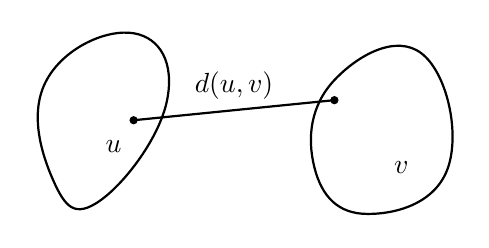
\begin{tikzpicture}[scale=0.85]
  % Blob u
  \draw[thick] plot [smooth cycle, tension=0.8] coordinates {(0,0) (1,1.5) (0.5,2.5) (-0.8,1.8) (-0.7,0.3)};
  \node at (0.2,0.8) {$u$};
  \coordinate (Pu) at (0.5,1.2);
  \filldraw (Pu) circle (1.5pt);
  
  % Blob v
  \draw[thick] plot [smooth cycle, tension=0.8] coordinates {(4,-0.2) (5.2,0.5) (4.8,2.2) (3.5,1.8) (3.2,0.5)};
  \node at (4.5,0.5) {$v$};
  \coordinate (Pv) at (3.5,1.5);
  \filldraw (Pv) circle (1.5pt);
  
  \draw[thick] (Pu) -- (Pv) node[midway, above] {$d(u, v)$};
\end{tikzpicture}
\caption{兩空間集合間的距離}
\label{fig:5-6}
\end{figure}

第四章已學了在平面上利用直線方程式來求點到直線的距離．下面命題給出了利用向量內積不僅在平面上，而且在空間中亦能求算點線距離的方法．

\begin{example}[論例 2]
在直線 $L$ 上任取一點 $B$，設 $\mathbf{a} = \vec{BA}$，而 $\mathbf{b}$ 為平行於 $L$ 的一個向量，則
\[ d(A, L) = \left| \mathbf{a} - \frac{\mathbf{a} \cdot \mathbf{b}}{|\mathbf{b}|^2} \mathbf{b} \right| \]
\end{example}

\begin{figure}[H]
\centering
\begin{tikzpicture}[scale=1.0]
  \coordinate (B) at (3.5,2.0);
  \coordinate (A) at (0,2.0);
  \coordinate (B0) at (1.5,0.7);
  
  \draw[thick] (-0.5,-0.7) -- (4.5,2.7) node[below right] {$L$};
  \draw[thick, -{Stealth}] (B) -- (A) node[midway, above] {$\mathbf{a}$};
  \draw[thick, -{Stealth}] (B) -- ++(-1.0,-0.7) node[below left] {$\mathbf{b}$};
  \draw[thick, -{Stealth}] (B0) -- (A) node[midway, left] {$\mathbf{a}_0$};
  
  \filldraw (A) circle (1.5pt) node[above] {$A$};
  \filldraw (B) circle (1.5pt) node[below right] {$B$};
  \filldraw (B0) circle (1.5pt) node[below right] {$B_0$};
  
  % Right angle mark at B0
  \draw[thin] ($(B0)+(0.12,0.15)$) -- ++(-0.15,0.12) -- ++(-0.12,-0.15);
\end{tikzpicture}
\caption{空間中點到直線距離之向量幾何計算}
\label{fig:5-7}
\end{figure}

\begin{proof}[證明]
設 $\mathbf{a}_0 = \vec{B_0A}$，則 $\mathbf{a}_0 = \vec{B_0A} = \vec{B_0B} + \vec{BA} = \beta \mathbf{b} + \mathbf{a}$，其中 $\beta$ 為一適當實數．
但 $\overline{AB_0} \perp L$，故 $\mathbf{a}_0 \cdot \mathbf{b} = 0$
卽 $(\beta \mathbf{b} + \mathbf{a}) \cdot \mathbf{b} = 0$，卽 $\beta = -\frac{\mathbf{a} \cdot \mathbf{b}}{|\mathbf{b}|^2}$
因此 $d(A, L) = |\mathbf{a}_0| = \left| \mathbf{a} - \frac{\mathbf{a} \cdot \mathbf{b}}{|\mathbf{b}|^2} \mathbf{b} \right|$ 故得證．
\end{proof}

此式其實不必記憶，需用時只要想一下我們老早提過的投影，$d(A, L)$ 就是垂線的長 $|\mathbf{a}_0|$，而 $\mathbf{a}_0$ 就是 $\mathbf{a}$ 減去 $\mathbf{a}$ 自己在 $L$ 線上的投影，但 $\mathbf{b}$ 既然是平行於 $L$，則 $\frac{\mathbf{b}}{|\mathbf{b}|}$ 便是平行於 $L$ 的單位向量，故上述投影量應為 $\mathbf{a} \cdot \frac{\mathbf{b}}{|\mathbf{b}|}$，而投影向量便是
\[ \left( \mathbf{a} \cdot \frac{\mathbf{b}}{|\mathbf{b}|} \right) \frac{\mathbf{b}}{|\mathbf{b}|} \]
卽
\[ d(A, L) = |\mathbf{a}_0| = \left| \mathbf{a} - \frac{\mathbf{a} \cdot \mathbf{b}}{|\mathbf{b}|^2} \mathbf{b} \right| \]

\begin{example}[例 2]
設根據一正交座標系 $(O; \mathbf{e}_1, \mathbf{e}_2, \mathbf{e}_3)$，有點 $A(-1, 5, 3)$，而 $L$ 為通過點 $B(0, 1, 1)$，點 $C(1, 2, 4)$ 的直線，求 $A$ 到 $L$ 的距離 $d(A, L)$．
\end{example}
\begin{proof}[解]
取 $\mathbf{a} = \vec{BA} = (-1, 4, 2)$，$\mathbf{b} = \vec{BC} = (1, 1, 3)$
則 $\mathbf{a} \cdot \mathbf{b} = -1 + 4 + 6 = 9$
$|\mathbf{b}|^2 = \mathbf{b} \cdot \mathbf{b} = 1 + 1 + 9 = 11$
因此
\begin{align*}
d(A, L) &= \left| \mathbf{a} - \frac{\mathbf{a} \cdot \mathbf{b}}{|\mathbf{b}|^2} \mathbf{b} \right| \\
&= \left| (-1, 4, 2) - \frac{9}{11}(1, 1, 3) \right| \\
&= \left| 5\left( \frac{-4}{11}, \frac{7}{11}, \frac{-1}{11} \right) \right| \\
&= 5 \sqrt{\frac{6}{11}}.
\end{align*}
這是直接代公式得出的結果．其實可以直接來求算，不必硬記公式

\begin{figure}[H]
\centering
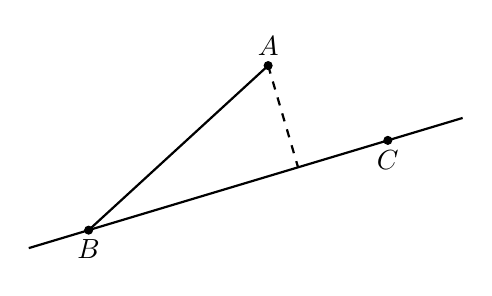
\begin{tikzpicture}[scale=0.95]
  \coordinate (B) at (0,0);
  \coordinate (C) at (4,1.2);
  \coordinate (A) at (2.4,2.2);
  \coordinate (H) at (2.8,0.84);
  
  \draw[thick] (-0.8,-0.24) -- (5.0,1.5);
  \draw[thick] (B) -- (A);
  \draw[thick, dashed] (A) -- (H);
  
  \filldraw (A) circle (1.5pt) node[above] {$A$};
  \filldraw (B) circle (1.5pt) node[below] {$B$};
  \filldraw (C) circle (1.5pt) node[below] {$C$};
\end{tikzpicture}
\caption{點到直線距離的直角三角形投影}
\label{fig:5-8}
\end{figure}

\[ \mathbf{a} = \vec{BA} = (-1, 4, 2),\quad \mathbf{b} = \vec{BC} = (1, 1, 3) \]
設 $\mathbf{a}_0 = \mathbf{a} - \beta \mathbf{b}$，而且 $\mathbf{a}_0$ 與 $\mathbf{b}$ 互相垂直
則 $\mathbf{a}_0 \cdot \mathbf{b} = 0 = (\mathbf{a} - \beta \mathbf{b}) \cdot \mathbf{b} = \mathbf{a} \cdot \mathbf{b} - \beta \mathbf{b} \cdot \mathbf{b}$
所以 $\beta = \frac{\mathbf{a} \cdot \mathbf{b}}{\mathbf{b} \cdot \mathbf{b}} = \frac{9}{11}$
\[ \mathbf{a}_0 = (-1, 4, 2) - \frac{9}{11}(1, 1, 3) = \frac{5}{11}(-4, 7, -1) \]
\[ d(A, L) = |\mathbf{a}_0| = 5 \sqrt{\frac{6}{11}} \]
\end{proof}

\begin{example}[論例 3]
設 $P$ 是經過 $B$ 點的平面，$\mathbf{b}, \mathbf{c}$ 是平面 $P$ 上兩個線性無關的向量，$A$ 不是 $P$ 上的點，$\mathbf{a} = \vec{BA}$，試以向量 $\mathbf{a}, \mathbf{b}, \mathbf{c}$ 表示 $d(A, P)$．
\end{example}

\begin{figure}[H]
\centering
\begin{tikzpicture}[scale=0.95]
  % Plane P
  \draw[thick] (0,0.5) -- (4,0) -- (6,2.5) -- (2,3.0) -- cycle;
  \node at (0.5,0.7) {$P$};
  
  \coordinate (B) at (1.5,1.0);
  \coordinate (A) at (3.5,3.8);
  \coordinate (H) at (3.5,1.5);
  \coordinate (b0) at (3.5,1.5);
  
  \filldraw (B) circle (1.5pt) node[below left] {$B$};
  \filldraw (A) circle (1.5pt) node[above right] {$A$};
  
  \draw[thick, -{Stealth}] (B) -- (A) node[midway, left] {$\mathbf{a}$};
  \draw[thick, -{Stealth}] (B) -- ++(1.5,0.5) node[above] {$\mathbf{b}$};
  \draw[thick, -{Stealth}] (B) -- ++(2.2,0.0) node[below] {$\mathbf{c}$};
  
  \draw[thick, -{Stealth}] (B) -- (H) node[midway, above] {$\mathbf{b}_0$};
  \draw[thick, dashed] (A) -- (H) node[midway, right] {$\mathbf{a}_0$};
\end{tikzpicture}
\caption{點到平面之距離向量分量}
\label{fig:5-9}
\end{figure}

\begin{proof}[解]
設 $\mathbf{b}_0 = \beta \mathbf{b} + \gamma \mathbf{c}$ 為平面 $P$ 上一向量，使得 $\mathbf{a} = \mathbf{a}_0 + \mathbf{b}_0$，$\mathbf{a}_0 = \mathbf{a} - \beta \mathbf{b} - \gamma \mathbf{c}$．
假設 $\mathbf{a}_0$ 與 $P$ 互相垂直，則 $\mathbf{a}_0$ 與 $\mathbf{b}$ 和 $\mathbf{c}$ 互相垂直，故有
\begin{align*}
\mathbf{a}_0 \cdot \mathbf{b} &= 0 = \mathbf{a} \cdot \mathbf{b} - \beta \mathbf{b} \cdot \mathbf{b} - \gamma \mathbf{c} \cdot \mathbf{b} \\
\mathbf{a}_0 \cdot \mathbf{c} &= 0 = \mathbf{a} \cdot \mathbf{c} - \beta \mathbf{b} \cdot \mathbf{c} - \gamma \mathbf{c} \cdot \mathbf{c}
\end{align*}
由
\[ \begin{cases} \beta \mathbf{b} \cdot \mathbf{b} + \gamma \mathbf{b} \cdot \mathbf{c} = \mathbf{a} \cdot \mathbf{b} \\ \beta \mathbf{b} \cdot \mathbf{c} + \gamma \mathbf{c} \cdot \mathbf{c} = \mathbf{a} \cdot \mathbf{c} \end{cases} \]
可以決定 $\beta$ 與 $\gamma$，從而可以算出 $d(A, P) = |\mathbf{a}_0|$ 的大小．
\end{proof}

\begin{example}[例 3]
設 $A = A(4, 2, 1)$，$B = B(-1, -1, 0)$，$C = C(0, 1, 2)$，$D = D(2, 1, 3)$，平面 $P$ 經過 $B, C, D$ 這三點，求 $d(A, P)$．
\end{example}
\begin{proof}[解]
$\vec{BA} = (5, 3, 1),\; \vec{BC} = (1, 2, 2),\; \vec{BD} = (3, 2, 3)$
設 $\mathbf{a} = \vec{BA} - \beta \vec{BC} - \gamma \vec{BD}$

\begin{figure}[H]
\centering
\begin{tikzpicture}[scale=0.85]
  % 3D Axes
  \draw[thick, -{Stealth}] (0,0) -- (0,4.0) node[above] {$z$};
  \draw[thick, -{Stealth}] (0,0) -- (5.0,0) node[right] {$y$};
  \draw[thick, -{Stealth}] (0,0) -- (-3.0,-2.0) node[below left] {$x$};
  
  \node at (0.3,0.3) {$O$};
  
  % Points B, C, D, A
  \coordinate (B) at (-0.5,-0.5);
  \coordinate (C) at (0.5,1.2);
  \coordinate (D) at (-0.3,1.8);
  \coordinate (A) at (-1.5,-0.8);
  
  \draw[thick] (B) -- (C) -- (D) -- cycle;
  \filldraw (B) circle (1.5pt) node[below left] {$B$};
  \filldraw (C) circle (1.5pt) node[above right] {$C$};
  \filldraw (D) circle (1.5pt) node[above left] {$D$};
  \filldraw (A) circle (1.5pt) node[below left] {$A$};
  
  % Plane outline
  \draw[thin] (-2.5,-1.2) -- (2.0,-0.8) -- (1.0,2.2) -- (-3.5,1.8) -- cycle;
  \draw[thick, dashed] (A) -- (-0.8,0.5);
\end{tikzpicture}
\caption{空間中點至平面之垂直投影}
\label{fig:5-10}
\end{figure}

\begin{align*}
&= (5, 3, 1) - \beta(1, 2, 2) - \gamma(3, 2, 3) \\
&= (5 - \beta - 3\gamma,\; 3 - 2\beta - 2\gamma,\; 1 - 2\beta - 3\gamma)
\end{align*}
與 $P$ 互相垂直\phantomsection\label{note:b3-ch5-p236-bd-prime}\footnote{【原書註記/校訂】：原書印作「$\mathbf{a} \cdot \vec{BD}' = 0$」，向量上方多出一撇，實為 $\vec{BD}$ 之印刷瑕疵，此處予以校訂．}
\begin{align*}
\therefore\quad &\mathbf{a} \cdot \vec{BC} = 0 = 13 - 9\beta - 13\gamma \\
&\mathbf{a} \cdot \vec{BD} = 0 = 24 - 13\beta - 22\gamma
\end{align*}
得
\[ \begin{cases} 9\beta + 13\gamma = 13 \\ 13\beta + 22\gamma = 24 \end{cases} \]
\[ \therefore\quad \gamma = \frac{47}{29},\quad \beta = \frac{-26}{29} \]
\begin{align*}
\mathbf{a} &= (5, 3, 1) + \frac{26}{29}(1, 2, 2) - \frac{47}{29}(3, 2, 3) \\
&= \frac{15}{29}(2, 3, -4)
\end{align*}
\[ \therefore\quad d(A, P) = |\mathbf{a}| = \frac{15}{29} |(2, 3, -4)| = \frac{15}{\sqrt{29}}. \]
\end{proof}

\begin{example}[例 4]
在正交座標平面上，點 $P(x_1, y_1)$ 到直線 $ax + by + c = 0$ 的距離為何？
\end{example}
\begin{proof}[解]
設 $Q(x_0, y_0)$ 為直線 $L : ax + by + c = 0$ 上之點，$\mathbf{u} = (a, b)$ 為 $L$ 之法線方向向量．則
$\left| \frac{\vec{QP} \cdot \mathbf{u}}{|\mathbf{u}|} \right|$ 為 $\vec{QP}$ 在 $L$ 之法線上之投影量，卽為點 $P$ 到 $L$ 之距離．

\begin{figure}[H]
\centering
\begin{tikzpicture}[scale=0.95]
  % Line L
  \draw[thick] (-1,0.5) -- (5,2.0);
  \coordinate (Q) at (0.5,0.9);
  \coordinate (P) at (2.5,3.2);
  \coordinate (R) at (3.0,1.5);
  
  \draw[thick] (Q) -- (P);
  \draw[thick] (P) -- (R);
  
  \filldraw (P) circle (1.5pt) node[above] {$P(x_1, y_1)$};
  \filldraw (Q) circle (1.5pt) node[below] {$Q(x_0, y_0)$};
  \filldraw (R) circle (1.5pt) node[below right] {$R$};
  
  % Right angle mark at R
  \draw[thin] ($(R)+(-0.15,0.25)$) -- ++(-0.25,-0.06) -- ++(0.15,-0.25);
\end{tikzpicture}
\caption{法線向量與點到直線距離}
\label{fig:5-11}
\end{figure}

由內積運算可得
\[ d(P, L) = \left| \frac{(x_1 - x_0, y_1 - y_0) \cdot (a, b)}{\sqrt{a^2 + b^2}} \right| = \frac{|ax_1 + by_1 + c|}{\sqrt{a^2 + b^2}}. \]
\end{proof}

\subsubsection*{作業 2}
\begin{enumerate}[label=(\roman*), leftmargin=2.5em]
  \item 求原點 $O$ 到 $3x + 2y + 1 = 0$ 的距離．
  \item 仿照例 4，證明點 $P(x_0, y_0, z_0)$ 與平面 $ax + by + cz + d = 0$ 的距離為
  \[ \frac{|ax_0 + by_0 + cz_0 + d|}{\sqrt{a^2 + b^2 + c^2}}. \]
  \item 求 $P(0, 4, 0)$ 至平面 $2x - y + 2z = 0$ 的距離．
\end{enumerate}

\subsubsection*{作業 3}
設根據一正交座標系 $(O; \mathbf{e}_1, \mathbf{e}_2, \mathbf{e}_3)$
\begin{enumerate}[label=(\roman*), leftmargin=2.5em]
  \item $A = A(3, 1, 1)$，直線 $L$ 通過 $(0, 1, 0), (0, 1, 1)$．
  \item $A = A(0, 0, 2)$，直線 $L$ 通過 $(1, 0, 0), (1, 3, 3)$．
\end{enumerate}
在每一小題上求 $d(A, L)$．

\subsubsection*{作業 4}
$\vec{AB} = (2, 1, 1),\; \vec{AC} = (0, 5, 4)$，試問以 $AB, AC$ 為一雙鄰邊做一平行四邊形 $ABDC$，求其面積．（提示：求 $B$ 至 $AC$ 距離）

\begin{figure}[H]
\centering
\begin{tikzpicture}[scale=0.65]
  % 3D Grid / Frame
  \draw[thick, -{Stealth}] (0,0) -- (0,5.5) node[above] {$z$};
  \draw[thick, -{Stealth}] (0,0) -- (6.0,0) node[right] {$y$};
  \draw[thick, -{Stealth}] (0,0) -- (-2.5,-2.0) node[below left] {$x$};
  
  \coordinate (A) at (0,0);
  \coordinate (B) at (-1.0, 1.5);
  \coordinate (C) at (3.5, 3.0);
  \coordinate (D) at ($(B)+(C)$);
  
  \draw[thick] (A) -- (B) -- (D) -- (C) -- cycle;
  \filldraw (A) circle (1.5pt) node[below left] {$A(0,0,0)$};
  \filldraw (B) circle (1.5pt) node[left] {$B(2,1,1)$};
  \filldraw (C) circle (1.5pt) node[above right] {$C(0,5,4)$};
  \filldraw (D) circle (1.5pt) node[above right] {$D$};
  
  % Grid hints
  \draw[dashed, thin] (0,0) grid[xstep=0.7, ystep=0.7] (3.5,3.0);
\end{tikzpicture}
\caption{以空間兩向量為鄰邊之平行四邊形}
\label{fig:5-12}
\end{figure}

\subsubsection*{作業 5}
設根據一正交座標系 $(O; \tilde{\mathbf{e}}_1, \tilde{\mathbf{e}}_2, \tilde{\mathbf{e}}_3)$
\begin{enumerate}[label=(\roman*), leftmargin=2.5em]
  \item $A = A(1, 0, 0)$，平面 $P$ 經過 $(7, 3, 4), (1, 0, 6), (4, 5, -2)$．
  \item $A = A(0, 1, 0)$，平面 $P$ 經過 $(6, 7, 3), (0, 3, 4), (-3, 7, 2)$．
\end{enumerate}
試求 $d(A, P)$．

\subsubsection*{作業 6}
求下列平面至點之距離．
\begin{enumerate}[label=(\roman*), leftmargin=2.5em]
  \item $4x + y + 8z + 39 = 0$，點：$(2, 2, 4)$
  \item $3x + 6y + 2z + 22 = 0$，點：$(1, 3, 3)$
  \item $2x + y + 2z = 0$，點：$(0, 6, 6)$
\end{enumerate}

\subsubsection*{作業 7}
$\vec{AB} = (1, 0, 2),\; \vec{AC} = (3, 1, 0),\; \vec{AD} = (2, 2, 2)$，以 $AB, AC, AD$ 為三鄰邊做一個平行六面體（如圖 5-13\phantomsection\label{note:b3-ch5-p238-fig-ref}\footnote{【原書註記/校訂】：原書印作「如圖 5-17」，而本頁下方對應平行六面體插圖編號實為「圖 5-13」．}），求此一平行六面體之體積．\\
（提示：$P$ 經過 $A, B, D$ 三點，先求 $C$ 至 $P$ 的距離．）

\begin{figure}[H]
\centering
\begin{tikzpicture}[scale=0.75]
  % 3D Frame
  \draw[thick, -{Stealth}] (0,0) -- (0,4.5) node[above] {$z$};
  \draw[thick, -{Stealth}] (0,0) -- (5.0,0) node[right] {$y$};
  \draw[thick, -{Stealth}] (0,0) -- (-2.5,-2.0) node[below left] {$x$};
  
  \coordinate (A) at (0,0);
  \coordinate (B) at (-0.5,1.5);
  \coordinate (C) at (1.5,0.0);
  \coordinate (D) at (0.8,1.2);
  
  \draw[thick] (A) -- (B);
  \draw[thick] (A) -- (C);
  \draw[thick] (A) -- (D);
  \draw[thick, dashed] (B) -- ($(B)+(C)$) -- (C);
  \draw[thick, dashed] (D) -- ($(D)+(B)$) -- ($(D)+(B)+(C)$) -- ($(D)+(C)$) -- cycle;
  \draw[thick, dashed] (B) -- ($(D)+(B)$);
  \draw[thick, dashed] ($(B)+(C)$) -- ($(D)+(B)+(C)$);
  \draw[thick, dashed] (C) -- ($(D)+(C)$);
  
  \filldraw (A) circle (1.5pt) node[below left] {$A$};
  \filldraw (B) circle (1.5pt) node[left] {$B$};
  \filldraw (C) circle (1.5pt) node[below] {$C$};
  \filldraw (D) circle (1.5pt) node[above right] {$D$};
\end{tikzpicture}
\caption{以空間三向量為鄰邊之平行六面體}
\label{fig:5-13}
\end{figure}

\subsubsection*{* 乙、直線與直線的距離}

今考慮兩條直線 $L_1, L_2$（共面或不共面不拘）之間距，記為 $d(L_1, L_2)$．若 $L_1$ 與 $L_2$ 相交時，$d(L_1, L_2) = 0$．如果不相交 $d(L_1, L_2) \neq 0$，此時分成 $L_1$ 與 $L_2$ 共面與不共面兩種狀況，圖示於後：

\begin{figure}[H]
\centering
\begin{subfigure}[b]{0.45\textwidth}
  \centering
  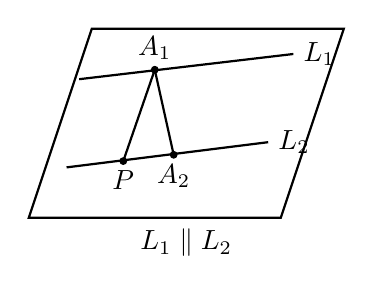
\begin{tikzpicture}[scale=0.8]
    % Plane
    \draw[thick] (0,0) -- (4,0) -- (5,3) -- (1,3) -- cycle;
    % L1 // L2
    \draw[thick] (0.8,2.2) -- (4.2,2.6) node[right] {$L_1$};
    \draw[thick] (0.6,0.8) -- (3.8,1.2) node[right] {$L_2$};
    \coordinate (A1) at (2.0,2.35);
    \coordinate (A2) at (2.3,1.0);
    \coordinate (P) at (1.5,0.9);
    \draw[thick] (A1) -- (A2);
    \draw[thick] (A1) -- (P);
    \filldraw (A1) circle (1.5pt) node[above] {$A_1$};
    \filldraw (A2) circle (1.5pt) node[below] {$A_2$};
    \filldraw (P) circle (1.5pt) node[below] {$P$};
    \node at (2.5,-0.4) {$L_1 \parallel L_2$};
  \end{tikzpicture}
\end{subfigure}
\hfill
\begin{subfigure}[b]{0.45\textwidth}
  \centering
  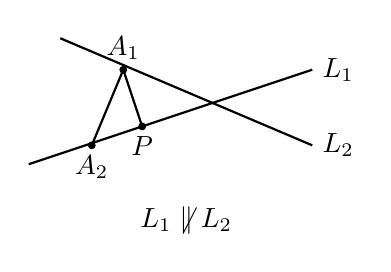
\begin{tikzpicture}[scale=0.8]
    \draw[thick] (0,0.5) -- (4.5,2.0) node[right] {$L_1$};
    \draw[thick] (0.5,2.5) -- (4.5,0.8) node[right] {$L_2$};
    \coordinate (A1) at (1.5,2.0);
    \coordinate (A2) at (1.0,0.8);
    \coordinate (P) at (1.8,1.1);
    \draw[thick] (A1) -- (A2);
    \draw[thick] (A1) -- (P);
    \filldraw (A1) circle (1.5pt) node[above] {$A_1$};
    \filldraw (A2) circle (1.5pt) node[below] {$A_2$};
    \filldraw (P) circle (1.5pt) node[below] {$P$};
    \node at (2.5,-0.4) {$L_1 \not\parallel L_2$};
  \end{tikzpicture}
\end{subfigure}
\caption{空間兩直線平行與相交情形}
\label{fig:5-14}
\end{figure}

如果有線段 $A_1A_2$，其中 $A_1, A_2$ 分別在 $L_1, L_2$ 上，它的長度
\[ \overline{A_1A_2} = d(L_1, L_2) \]
我們要證明直線 $A_1A_2$ 必須同時垂直於 $L_1$ 與 $L_2$（此時稱 $A_1A_2$ 為 $L_1$ 與 $L_2$ 的公垂線）．

若 $A_1A_2$ 不是 $L_1$ 與 $L_2$ 的公垂線，設 $A_1A_2$ 不垂直於 $L_2$，則在 $L_2$ 上靠近 $A_2$ 的地方取一點 $P$，使得 $\angle A_1A_2P$ 為一銳角，而 $\angle A_1PA_2$ 則為鈍角．由於大角對大邊知得
\[ \overline{A_1A_2} > \overline{A_1P} \]
故 $A_1A_2$ 不可能為 $L_1$ 上的點到 $L_2$ 上的點間的最短距離．此與 $\overline{A_1A_2} = d(L_1, L_2)$ 的假設不符．因此得證 $A_1A_2$ 必為 $L_1$ 與 $L_2$ 的公垂線．

\begin{figure}[H]
\centering
\begin{tikzpicture}[scale=0.95]
  % Skew lines L1 and L2
  \draw[thick] (0,2.5) -- (5.0,0.5) node[right] {$L_1$};
  \draw[thick] (0,-0.5) -- (5.0,1.5) node[right] {$L_2$};
  
  \coordinate (A1) at (1.5,1.9);
  \coordinate (A2) at (1.2,0.0);
  \draw[thick] (A1) -- (A2);
  \filldraw (A1) circle (1.5pt) node[above] {$A_1$};
  \filldraw (A2) circle (1.5pt) node[below] {$A_2$};
  
  \coordinate (B1) at (3.5,1.1);
  \coordinate (B2) at (2.5,0.5);
  \filldraw (B1) circle (1.5pt) node[above right] {$B_1$};
  \filldraw (B2) circle (1.5pt) node[below] {$B_2$};
  
  \draw[thick, -{Stealth}] (B1) -- ++(1.0,-0.4) node[below] {$\mathbf{b}_1$};
  \draw[thick, -{Stealth}] (B2) -- ++(1.0,0.4) node[below] {$\mathbf{b}_2$};
  \draw[thick] (B2) -- (B1) node[midway, left] {$\mathbf{a}$};
  \draw[thick] (A2) -- (A1) node[midway, right] {$\mathbf{a}_0$};
\end{tikzpicture}
\caption{歪斜直線與公垂線向量分解}
\label{fig:5-15}
\end{figure}

接著，我們就藉所算出公垂線的長度 $\overline{A_1A_2}$ 來求 $d(L_1, L_2)$．

\begin{prop}
\label{prop:b3-5-3}
設向量 $\mathbf{a}_0 = \vec{A_1A_2}$，其中 $A_1A_2$ 為直線 $L_1$ 與 $L_2$ 的公垂線，設 $\mathbf{b}_1, \mathbf{b}_2$ 分別為平行於 $L_1, L_2$ 的兩個單位向量（$|\mathbf{b}_1| = |\mathbf{b}_2| = 1$），而 $\mathbf{a}$ 為 $L_1$ 上任一點 $B_1$ 到 $L_2$ 上任一點 $B_2$ 的有向線段所代表的向量．

則 $d(L_1, L_2) = |\mathbf{a}_0| = |\mathbf{a} + \beta_1 \mathbf{b}_1 + \beta_2 \mathbf{b}_2|$，其中
\begin{align}
\beta_1 &= \frac{(\mathbf{a} \cdot \mathbf{b}_2)(\mathbf{b}_2 \cdot \mathbf{b}_1) - (\mathbf{a} \cdot \mathbf{b}_1)}{1 - (\mathbf{b}_1 \cdot \mathbf{b}_2)^2}, \notag \\
\beta_2 &= \frac{(\mathbf{a} \cdot \mathbf{b}_1)(\mathbf{b}_1 \cdot \mathbf{b}_2) - (\mathbf{a} \cdot \mathbf{b}_2)}{1 - (\mathbf{b}_1 \cdot \mathbf{b}_2)^2} \label{eq:b3-5-7}
\end{align}
\end{prop}

\begin{proof}[證明]
這裏的基本觀念與論例 2 的沒有區別．先計算一下 $\mathbf{a}_0$：
\begin{equation}
\mathbf{a}_0 = \vec{A_1A_2} = \vec{A_1B_1} + \vec{B_1B_2} + \vec{B_2A_2} = \beta_1 \mathbf{b}_1 + \mathbf{a} + \beta_2 \mathbf{b}_2 \label{eq:b3-5-8}
\end{equation}
（如圖 5-15\phantomsection\label{note:b3-ch5-p240-fig-ref}\footnote{【原書註記/校訂】：原書印作「（如圖 5-19）」，而對應之公垂線幾何圖實際編號為「圖 5-15」．}）其中 $\beta_1, \beta_2$ 為未定的兩實數（可正可負，以調整一開始 $\mathbf{b}_1, \mathbf{b}_2$ 之分別與 $\vec{A_1B_1}, \vec{B_2A_2}$ 是否同向）．$\beta_1$ 與 $\beta_2$ 的決定可由下列代表 $A_1A_2$ 為公垂線的兩條件給出：
\[ \begin{cases} \mathbf{a}_0 \cdot \mathbf{b}_1 = 0 & [A_1A_2 \perp L_1] \\ \mathbf{a}_0 \cdot \mathbf{b}_2 = 0 & [A_1A_2 \perp L_2] \end{cases} \]
將 \eqref{eq:b3-5-8} 式代入，得
\[ \begin{cases} \beta_1 \mathbf{b}_1 \cdot \mathbf{b}_1 + \mathbf{a} \cdot \mathbf{b}_1 + \beta_2 \mathbf{b}_2 \cdot \mathbf{b}_1 = 0 \\ \beta_1 \mathbf{b}_1 \cdot \mathbf{b}_2 + \mathbf{a} \cdot \mathbf{b}_2 + \beta_2 \mathbf{b}_2 \cdot \mathbf{b}_2 = 0 \end{cases} \]
卽
\[ \begin{cases} \beta_1 + \beta_2 (\mathbf{b}_2 \cdot \mathbf{b}_1) = -\mathbf{a} \cdot \mathbf{b}_1 \\ \beta_1 (\mathbf{b}_1 \cdot \mathbf{b}_2) + \beta_2 = -\mathbf{a} \cdot \mathbf{b}_2 \end{cases} \]
根據第一冊聯立方程式之解得
\[ \beta_1 = \frac{\begin{vmatrix} -\mathbf{a} \cdot \mathbf{b}_1 & \mathbf{b}_2 \cdot \mathbf{b}_1 \\ -\mathbf{a} \cdot \mathbf{b}_2 & 1 \end{vmatrix}}{\begin{vmatrix} 1 & \mathbf{b}_2 \cdot \mathbf{b}_1 \\ \mathbf{b}_1 \cdot \mathbf{b}_2 & 1 \end{vmatrix}},\quad \beta_2 = \frac{\begin{vmatrix} 1 & -\mathbf{a} \cdot \mathbf{b}_1 \\ \mathbf{b}_1 \cdot \mathbf{b}_2 & -\mathbf{a} \cdot \mathbf{b}_2 \end{vmatrix}}{\begin{vmatrix} 1 & \mathbf{b}_2 \cdot \mathbf{b}_1 \\ \mathbf{b}_1 \cdot \mathbf{b}_2 & 1 \end{vmatrix}} \]
卽得 \eqref{eq:b3-5-7} 式．
\end{proof}

\begin{example}[例 5]
設直線 $L_1$ 經過 $A(0, 4, 2), B(1, 5, 2)$；直線 $L_2$ 經過 $C(0, 1, 0), D(2, 1, 1)$；求 $L_1$ 與 $L_2$ 的距離．
\end{example}

\begin{figure}[H]
\centering
\begin{tikzpicture}[scale=0.95]
  \coordinate (A) at (0.5,3.0);
  \coordinate (B) at (3.0,2.3);
  \coordinate (C) at (0.5,0.5);
  \coordinate (D) at (2.5,1.5);
  
  \draw[thick] (-0.5,3.3) -- (4.5,1.9) node[right] {$L_1$};
  \draw[thick] (-0.5,0.0) -- (4.5,2.5) node[right] {$L_2$};
  
  \filldraw (A) circle (1.5pt) node[above] {$A(0,4,2)$};
  \filldraw (B) circle (1.5pt) node[above] {$B(1,5,2)$};
  \filldraw (C) circle (1.5pt) node[below] {$C(0,1,0)$};
  \filldraw (D) circle (1.5pt) node[below] {$D(2,1,1)$};
  
  \draw[thick] (A) -- (C);
  \coordinate (A1) at (2.0,2.6);
  \coordinate (A2) at (2.0,1.25);
  \draw[thick, -{Stealth}] (A1) -- (A2);
  \filldraw (A1) circle (1.5pt) node[above right] {$A_1$};
  \filldraw (A2) circle (1.5pt) node[below right] {$A_2$};
\end{tikzpicture}
\caption{空間兩直線公垂線段距離計算}
\label{fig:5-16}
\end{figure}

\begin{proof}[解]
$\vec{AB} = (1, 1, 0),\; \vec{CD} = (2, 0, 1),\; \vec{CA} = (0, 3, 2)$
設 $\vec{A_1A_2}$ 為 $L_1$ 與 $L_2$ 的公垂線，垂足為 $A_1, A_2$，
則 $L_1$ 與 $L_2$ 的距離為 $|\vec{A_1A_2}|$
\[ \vec{A_1A_2} = \beta \vec{AB} - \vec{CA} + \gamma \vec{CD} \quad \text{在此 } \beta, \gamma \text{ 為未知數．} \]
而且 $\vec{A_1A_2} \cdot \vec{AB} = 0,\; \vec{A_1A_2} \cdot \vec{CD} = 0$
$\therefore\quad \vec{A_1A_2} = (\beta + 2\gamma,\; \beta - 3,\; \gamma - 2)$
\begin{align*}
\vec{A_1A_2} \cdot \vec{AB} &= 0 = 2\beta + 2\gamma - 3 \\
\vec{A_1A_2} \cdot \vec{CD} &= 0 = 2\beta + 5\gamma - 2
\end{align*}
$\therefore\quad \begin{cases} 2\beta + 2\gamma = 3 \\ 2\beta + 5\gamma = 2 \end{cases}$ \\
$\therefore\quad \gamma = \frac{-1}{3},\quad \beta = \frac{11}{6}$ \\
$\therefore\quad \vec{A_1A_2} = \left( \frac{7}{6}, \frac{-7}{6}, \frac{-7}{3} \right) = \frac{7}{6}(1, -1, -2)$ \\
所以 $L_1$ 與 $L_2$ 的距離為 $|\vec{A_1A_2}| = \frac{7}{6}\sqrt{6}$．
\end{proof}

\noindent\textbf{注意}\quad 命題 3 所導出的公式不需要背，正如同一上面這一個例題可以直接計算，所用的只是那一個方法．

上述求公垂線的長度，在工程上是常常要應用的，要張撐兩根屋樑的最穩定的方法是在公垂線的位置上支撐一根柱子，那麼若知道這兩根橫樑的位置，就可求得這根柱子的長．（見下例）

\begin{example}[例 6]
如圖 5-17\phantomsection\label{note:b3-ch5-p242-fig-ref}\footnote{【原書註記/校訂】：原書印作「如圖 5-21」，而本頁右側之屋樑與柱子插圖實際編號為「圖 5-17」．}，設 $P_1$ 與 $P_2$ 為互相平行的兩面牆，$\overline{AB}$ 是一根水平的橫樑，假設 $\overline{AB}$ 垂直 $P_1$，由 $A$ 向下 3 公尺，向後 2 公尺，得 $C$ 點；由 $B$ 向下 7 公尺，向前 5 公尺，得 $D$ 點；再架一根橫樑 $\overline{CD}$，求 $\overline{AB}$ 與 $\overline{CD}$ 的距離，設 $\overline{AB}$ 的長度為 10 公尺．
\end{example}

\begin{figure}[H]
\centering
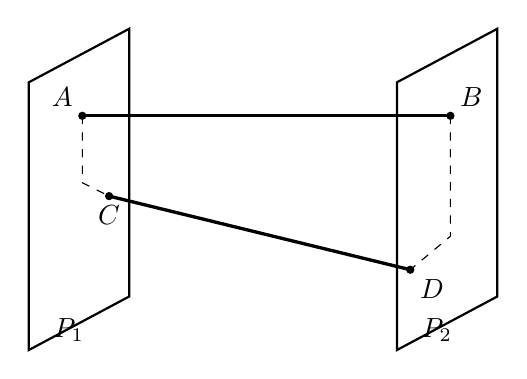
\begin{tikzpicture}[scale=0.85]
  % Wall P1
  \draw[thick] (0,0) -- (0,4.0) -- (1.5,4.8) -- (1.5,0.8) -- cycle;
  \node at (0.6,0.3) {$P_1$};
  % Wall P2
  \draw[thick] (5.5,0) -- (5.5,4.0) -- (7.0,4.8) -- (7.0,0.8) -- cycle;
  \node at (6.1,0.3) {$P_2$};
  
  % Beam AB
  \coordinate (A) at (0.8,3.5);
  \coordinate (B) at (6.3,3.5);
  \draw[very thick] (A) -- (B);
  \filldraw (A) circle (1.5pt) node[above left] {$A$};
  \filldraw (B) circle (1.5pt) node[above right] {$B$};
  
  % Point C
  \coordinate (C) at (1.2,2.3);
  \filldraw (C) circle (1.5pt) node[below] {$C$};
  \draw[dashed] (A) -- ++(0,-1.0) -- (C);
  
  % Point D
  \coordinate (D) at (5.7,1.2);
  \filldraw (D) circle (1.5pt) node[below right] {$D$};
  \draw[dashed] (B) -- ++(0,-1.8) -- (D);
  
  % Beam CD
  \draw[very thick] (C) -- (D);
\end{tikzpicture}
\caption{平行牆面與交叉橫樑結構}
\label{fig:5-17}
\end{figure}

\begin{proof}[解]
令 $OH$ 與 $AB$ 平行，以 $O$ 為原點 $OH$ 為 $x$ 軸，$OC$ 為 $y$ 軸，$OA$ 為 $z$ 軸．
\begin{align*}
A &= A(0, 0, 3) \\
C &= C(0, 2, 0) \\
B &= B(10, 0, 3) \\
D &= D(10, -5, -4) \\
\vec{AB} &= (10, 0, 0) \\
\vec{CD} &= (10, -7, -4) \\
\vec{CA} &= (0, -2, 3)
\end{align*}

\begin{figure}[H]
\centering
\begin{tikzpicture}[scale=0.85]
  % 3D Axes
  \draw[thick, -{Stealth}] (0,0) -- (0,3.8) node[above] {$z$};
  \draw[thick, -{Stealth}] (0,0) -- (6.5,0) node[right] {$x$};
  \draw[thick, -{Stealth}] (0,0) -- (4.5,2.6) node[above right] {$y$};
  
  \node at (-0.3,-0.2) {$O$};
  
  \coordinate (A) at (0,2.4);
  \coordinate (C) at (1.8,1.0);
  \coordinate (B) at (5.0,2.4);
  \coordinate (H) at (5.0,0);
  \coordinate (G) at (5.0,-1.8);
  \coordinate (D) at (3.8,-3.0);
  
  \draw[thick] (A) -- (B);
  \draw[thick] (C) -- (D);
  \draw[thick] (A) -- (C);
  \draw[dashed] (B) -- (H) -- (G) -- (D);
  
  \filldraw (A) circle (1.5pt) node[left] {$A(0,0,3)$};
  \filldraw (C) circle (1.5pt) node[above right] {$C(0,2,0)$};
  \filldraw (B) circle (1.5pt) node[above right] {$B(10,0,3)$};
  \filldraw (H) circle (1.5pt) node[above right] {$H$};
  \filldraw (G) circle (1.5pt) node[right] {$G$};
  \filldraw (D) circle (1.5pt) node[below] {$D(10,-5,-4)$};
  
  % Strut vector a
  \draw[thick, dashed, -{Stealth}] (2.5,2.4) -- (2.3,-0.8) node[midway, right] {$\mathbf{a}$};
\end{tikzpicture}
\caption{橫樑公垂線距離座標模型}
\label{fig:5-18}
\end{figure}

設 $\mathbf{a}$ 與 $\vec{AB}, \vec{CD}$ 互相垂直，而且 $\mathbf{a}$ 的長度剛好是 $\overline{AB}$ 與 $\overline{CD}$ 的距離．\\
令 $\mathbf{a} = \beta \vec{CD} + \vec{CA} + \gamma \vec{AB}$ \\
$\mathbf{a} \cdot \vec{AB} = 0,\quad \mathbf{a} \cdot \vec{CD} = 0$ \\
$\therefore\quad \mathbf{a} = (10\beta + 10\gamma,\; -7\beta - 2,\; -4\beta + 3)$ \\
$\therefore\quad \begin{cases} 100\beta + 100\gamma = 0 \\ 165\beta + 100\gamma + 2 = 0 \end{cases}$ \\
$\therefore\quad \beta = -\gamma$ \\
$\beta = \frac{-2}{65},\quad \gamma = \frac{2}{65}$ \\
$\mathbf{a} = \left( 0, \frac{-116}{65}, \frac{203}{65} \right) = \frac{29}{65}(0, -4, 7)$ \\
$\therefore\quad |\mathbf{a}| = \frac{29}{65}\sqrt{65} = \frac{29}{\sqrt{65}}$．
\end{proof}

\subsubsection*{作業 8}
\begin{enumerate}[label=(\roman*), leftmargin=2.5em]
  \item 設直線 $L_1$ 通過 $(0, -39, 0), (0, -7, -4)$；直線 $L_2$ 通過 $(2, 2, 4), (0, 0, 0)$．
  \item 設直線 $L_1$ 通過 $(0, 0, -11), (0, -3, 2)$；直線 $L_2$ 通過 $(1, 3, 3), (1, 1, 0)$．
\end{enumerate}
求 $L_1$ 與 $L_2$ 的距離．

\subsubsection*{作業 9}
求下列平面至直線的距離．
\begin{enumerate}[label=(\roman*), leftmargin=2.5em]
  \item $4x + y + 8z + 39 = 0$，直線 $L$ 通過 $(0, 0, 0), (-2, 0, 1)$．
  \item $3x + 6y + 2z + 22 = 0$，直線 $L$ 通過 $(-2, 1, 0), (-2, 0, 3)$．
\end{enumerate}
（提示：若所給直線與平面平行，則取直線上一點，求此點到平面之距離）

\subsubsection*{習題 5-2}
以下全採用正交座標系，且用向量表示．
\begin{enumerate}[leftmargin=2em]
  \item 試求點 $(2, 1)$ 到直線 $5x + 3y = 8$ 的距離．
  \item 試求點 $(1, 3, -1)$ 到平面 $2x + y - z = 4$ 的距離．
  \item 設直線 $L$ 通過 $(2, 1, 0)$ 與 $(0, 1, 1)$，求點 $A(2, 5, 2)$ 到 $L$ 的距離．
  \item 設平面 $P$ 經過 $(3, 6, -2), (7, -4, 3), (-1, 4, -7)$，試求點 $P(0, 0, 1)$ 到 $P$ 的距離．
  \item 設 $\vec{AB} = (a, b, c),\; \vec{AC} = (d, e, f)$，試問以 $AB, AC$ 為一雙鄰邊做一平行四邊形，其面積如何？
  \item 設 $\vec{AB} = (a, b, c),\; \vec{AC} = (d, e, f),\; \vec{AD} = (g, h, k)$，試求以 $AB, AC, AD$ 為三鄰邊所做出平行六面體的體積．
  \item 設直線 $L_1$ 通過 $(0, 0, 0), (-1, 0, 1)$，直線 $L_2$ 通過 $(-1, 2, 1), (1, 2, 1)$，試求 $L_1$ 與 $L_2$ 的距離．
  \item 求平面 $2x + y + 2z = 0$ 到直線 $L$ 之距離，$L$ 通過 $(-1, 0, 0), (0, -2, 0)$ 兩點．
\end{enumerate}

% ==========================================
% § 5-3 座標與向量進一步的混合運用
% ==========================================
\subsection{* 座標與向量進一步的混合運用}\label{sec:b3-5-3}

我們舉帕卜（Pappus）定理，歐拉（Euler）線，笛沙格（Desargues）定理來看：

如何混合運用座標與向量來處理這樣一些複雜的幾何問題．請特別注意這一節的要點不在於這些定理本身的陳述，只是借助它們把運用的方法顯示出來．

\begin{example}[論例 4]（帕卜 Pappus 定理）
在相交的兩直線 $L_1$ 與 $L_2$ 上，各取兩組點 $A_1, A_2, A_3$ 和 $B_1, B_2, B_3$，假定 $A_1B_2$ 與 $A_2B_1$，$A_1B_3$ 與 $A_3B_1$，$A_2B_3$ 與 $A_3B_2$ 各有唯一交點 $P, Q, R$，則 $P, Q, R$ 必定共線．
\end{example}

\begin{figure}[H]
\centering
\begin{tikzpicture}[scale=0.95]
  % Lines L1 and L2 intersecting at O
  \coordinate (O) at (0,0);
  \draw[thick] (-0.8,0.4) -- (6.5,-3.25) node[right] {$L_1$};
  \draw[thick] (-0.8,-0.14) -- (6.5,1.14) node[right] {$L_2$};
  \filldraw (O) circle (1.5pt) node[below left] {$O$};
  
  % Points on L1
  \coordinate (A1) at (1.2,-0.6);
  \coordinate (A2) at (2.4,-1.2);
  \coordinate (A3) at (5.0,-2.5);
  \filldraw (A1) circle (1.5pt) node[below left] {$A_1$};
  \filldraw (A2) circle (1.5pt) node[below left] {$A_2$};
  \filldraw (A3) circle (1.5pt) node[below left] {$A_3$};
  
  % Points on L2
  \coordinate (B1) at (2.0,0.35);
  \coordinate (B2) at (4.0,0.7);
  \coordinate (B3) at (5.8,1.015);
  \filldraw (B1) circle (1.5pt) node[above] {$B_1$};
  \filldraw (B2) circle (1.5pt) node[above] {$B_2$};
  \filldraw (B3) circle (1.5pt) node[above] {$B_3$};
  
  % Segments
  \draw (A1) -- (B2);
  \draw (A2) -- (B1);
  \draw (A1) -- (B3);
  \draw (A3) -- (B1);
  \draw (A2) -- (B3);
  \draw (A3) -- (B2);
  
  % Intersections P, Q, R
  \coordinate (P) at (intersection of A1--B2 and A2--B1);
  \coordinate (Q) at (intersection of A1--B3 and A3--B1);
  \coordinate (R) at (intersection of A2--B3 and A3--B2);
  
  \filldraw (P) circle (1.5pt) node[above left] {$P$};
  \filldraw (Q) circle (1.5pt) node[above] {$Q$};
  \filldraw (R) circle (1.5pt) node[above left] {$R$};
  
  % Dashed collinear line
  \draw[thick, dashed] ($(P)!-0.3!(R)$) -- ($(P)!1.3!(R)$);
\end{tikzpicture}
\caption{帕卜（Pappus）共線定理}
\label{fig:5-19}
\end{figure}

\noindent\textbf{注意}\quad 先多作一些圖，使得 $A_1, A_2, A_3$ 與 $B_1, B_2, B_3$ 可隨便在 $L_1, L_2$ 上散置，且不一定皆在 $O$ 的一側，試看看繪圖結果是否始終有著 $P, Q, R$ 共線的現象．

\begin{proof}[證明]
不妨假設 $A_1 \neq O,\; B_1 \neq O$．故取 $\tilde{\mathbf{e}}_1 = \vec{OA}_1,\; \tilde{\mathbf{e}}_2 = \vec{OB}_1$，則 $(O; \tilde{\mathbf{e}}_1, \tilde{\mathbf{e}}_2)$ 構成一個座標系．（$\tilde{\mathbf{e}}_1$ 與 $\tilde{\mathbf{e}}_2$ 為線性無關，因 $O, A_1, B_1$ 三點不共線）根據這一座標系，我們有座標：
\begin{align*}
A_1(1, 0),\quad &A_2(\alpha, 0),\quad A_3(\alpha', 0) \\
B_1(0, 1),\quad &B_2(0, \beta),\quad B_3(0, \beta')
\end{align*}
先看看 $R$ 點座標，直線 $A_2B_3$ 與直線 $A_3B_2$ 分別有向量參數表示式：
\begin{align}
\vec{OA}_2 + t(\vec{OB}_3 - \vec{OA}_2) &= \alpha \tilde{\mathbf{e}}_1 + t(\beta' \tilde{\mathbf{e}}_2 - \alpha \tilde{\mathbf{e}}_1) \label{eq:b3-5-9} \\
\text{與}\quad \vec{OA}_3 + s(\vec{OB}_2 - \vec{OA}_3) &= \alpha' \tilde{\mathbf{e}}_1 + s(\beta \tilde{\mathbf{e}}_2 - \alpha' \tilde{\mathbf{e}}_1) \label{eq:b3-5-10}
\end{align}
其中 $t$ 與 $s$ 分別為兩直線之參數．

$R$ 既然是這兩直線的交點，$\vec{OR}$ 便能同時表現為 \eqref{eq:b3-5-9} 與 \eqref{eq:b3-5-10} 式，稍為整理一下，得
\[ \alpha'(1 - s)\tilde{\mathbf{e}}_1 + s\beta \tilde{\mathbf{e}}_2 = \vec{OR} = \alpha(1 - t)\tilde{\mathbf{e}}_1 + t\beta'\tilde{\mathbf{e}}_2 \]
因 $\tilde{\mathbf{e}}_1$ 與 $\tilde{\mathbf{e}}_2$ 線性無關，故
\[ \begin{cases} \alpha'(1 - s) = \alpha(1 - t) \\ s\beta = t\beta' \end{cases} \]
解 $t$ 得
\[ t = \frac{\alpha\beta - \alpha'\beta}{\alpha\beta - \alpha'\beta'} = \frac{(\alpha - \alpha')\beta}{\alpha\beta - \alpha'\beta'} \]
故
\[ \vec{OR} = \alpha \tilde{\mathbf{e}}_1 + \frac{(\alpha - \alpha')\beta}{\alpha\beta - \alpha'\beta'}(\beta'\tilde{\mathbf{e}}_2 - \alpha \tilde{\mathbf{e}}_1) \]
故根據 $(O; \tilde{\mathbf{e}}_1, \tilde{\mathbf{e}}_2)$ 之座標系，$R$ 點的座標為
\begin{equation}
R\left( \frac{\alpha\alpha'(\beta - \beta')}{\alpha\beta - \alpha'\beta'},\; \frac{\beta\beta'(\alpha - \alpha')}{\alpha\beta - \alpha'\beta'} \right) \label{eq:b3-5-11}
\end{equation}
同理，可求得 $P, Q$ 的座標分別為
\begin{align*}
P\left( \frac{\alpha(\beta - 1)}{\alpha\beta - 1},\; \frac{\beta(\alpha - 1)}{\alpha\beta - 1} \right) \quad &\text{〔在 \eqref{eq:b3-5-11} 式中代 $\alpha' = \beta' = 1$〕} \\
Q\left( \frac{\alpha'(1 - \beta')}{1 - \alpha'\beta'},\; \frac{\beta'(1 - \alpha')}{1 - \alpha'\beta'} \right) \quad &\text{〔在 \eqref{eq:b3-5-11} 式中代 $\alpha = \beta = 1$〕}
\end{align*}
最後要證 $P, Q, R$ 為共線，卽欲證：
\[ \text{存在不全為 0 的實數 } a, b, c \text{ 使得 } a\vec{OP} + b\vec{OQ} + c\vec{OR} = \mathbf{0}\text{，且 } a + b + c = 0. \]
取 $a = \alpha'\beta'(1 - \alpha\beta),\; b = \alpha\beta(\alpha'\beta' - 1),\; c = \alpha\beta - \alpha'\beta'$，卽可予驗證．
\end{proof}

\begin{example}[論例 5]（歐拉 Euler 線）
$\triangle ABC$ 的外心 $O$，重心 $W$，垂心 $H$，三點共線．（這一事實是歐拉（Euler）所發現，所以稱為歐拉線．）
\end{example}
\begin{proof}[解]
過 $A$ 點做 $l_A \parallel BC$，過 $B$ 點做 $l_B \parallel AC$，過 $C$ 點做 $l_C \parallel AB$，$l_A, l_B, l_C$ 兩兩相交做成 $\triangle A'B'C'$，則 $\triangle ABC$ 的垂心 $H$ 也就是 $\triangle A'B'C'$ 的外心，以 $\triangle ABC$ 的重心 $W$ 為始點，設
$\mathbf{a} = \vec{WA},\; \mathbf{b} = \vec{WB},\; \mathbf{c} = \vec{WC}$，則由 § 4-6 論例知\phantomsection\label{note:b3-ch5-p247-sec-ref}\footnote{【原書註記/校訂】：原書印作「由 §4-6 論例知」，重心性質 $\vec{WA} + \vec{WB} + \vec{WC} = \mathbf{0}$ 實為 § 4-7 命題 3．正文保留原刊字樣並加註．}

\begin{figure}[H]
\centering
\begin{tikzpicture}[scale=0.95]
  % Triangle ABC
  \coordinate (A) at (2.2,3.2);
  \coordinate (B) at (1.0,0.5);
  \coordinate (C) at (5.0,0.5);
  
  % Anti-complementary Triangle A'B'C'
  \coordinate (Aprime) at ($(B)+(C)-(A)$);
  \coordinate (Bprime) at ($(A)+(C)-(B)$);
  \coordinate (Cprime) at ($(A)+(B)-(C)$);
  
  \draw[thick] (A) -- (B) -- (C) -- cycle;
  \draw[thick] (Aprime) -- (Bprime) -- (Cprime) -- cycle;
  
  % Lines lA, lB, lC labels
  \node at (4.0,3.5) {$l_A$};
  \node at (5.5,1.8) {$l_C$};
  \node at (2.3,-0.8) {$l_B$};
  
  % Points A, B, C, A', B', C'
  \filldraw (A) circle (1.5pt) node[above] {$A$};
  \filldraw (B) circle (1.5pt) node[below left] {$B$};
  \filldraw (C) circle (1.5pt) node[right] {$C$};
  \filldraw (Aprime) circle (1.5pt) node[below] {$A'$};
  \filldraw (Bprime) circle (1.5pt) node[above right] {$B'$};
  \filldraw (Cprime) circle (1.5pt) node[above left] {$C'$};
  
  % Centroid W
  \coordinate (W) at (barycentric cs:A=1,B=1,C=1);
  \filldraw (W) circle (1.5pt) node[below right] {$W$};
  
  % Orthocenter H
  \coordinate (H) at (1.5,1.3);
  \filldraw (H) circle (1.5pt) node[left] {$H$};
  
  % Circumcenter O
  \coordinate (O) at (3.0,1.3);
  \filldraw (O) circle (1.5pt) node[right] {$O$};
  
  % Vectors from W
  \draw[-{Stealth}] (W) -- (A) node[midway, left] {$\mathbf{a}$};
  \draw[-{Stealth}] (W) -- (B) node[midway, below] {$\mathbf{b}$};
  \draw[-{Stealth}] (W) -- (C) node[midway, above] {$\mathbf{c}$};
  
  % Dashed reflections to A', B', C'
  \draw[thick, dashed] (W) -- (Bprime) node[midway, above] {$-2\mathbf{b}$};
  \draw[thick, dashed] (W) -- (Cprime) node[midway, above left] {$-2\mathbf{c}$};
  \draw[thick, dashed] (W) -- (Aprime) node[midway, right] {$-2\mathbf{a}$};
  
  % Altitudes from vertices
  \draw[thin] (A) -- (2.2,0.5);
  \draw[thin] (B) -- (2.7,2.7);
  \draw[thin] (C) -- (1.5,1.8);
\end{tikzpicture}
\caption{歐拉（Euler）線幾何與向量反映}
\label{fig:5-20}
\end{figure}

\[ \frac{1}{3}(\mathbf{a} + \mathbf{b} + \mathbf{c}) = \vec{WW} = \mathbf{0} \quad \text{亦卽 } \mathbf{a} + \mathbf{b} + \mathbf{c} = \mathbf{0} \]
再者
\begin{align*}
\vec{WB}' &= \vec{WB} + \vec{BC} + \vec{CB}' \\
&= \mathbf{b} + (\mathbf{c} - \mathbf{b}) + (\mathbf{a} - \mathbf{b}) \\
&= (\mathbf{a} + \mathbf{b} + \mathbf{c}) - 2\mathbf{b} \quad \text{〔因 } \vec{CB}' = \vec{BA} = \mathbf{a} - \mathbf{b}\text{〕} \\
&= -2\mathbf{b}. \quad (\therefore B, W, B' \text{ 共線})
\end{align*}
同理可證 $\vec{WA}' = -2\mathbf{a},\; \vec{WC}' = -2\mathbf{c}$．($\therefore A, W, A'$ 及 $C, W, C'$ 各共線)

換句話說：$\triangle A'B'C'$ 是先把 $\triangle ABC$ 以 $W$ 點為中心作反映再延長 2 倍，卽得 $\triangle A'B'C'$ 的外心 $H$（亦卽 $\triangle ABC$ 的垂心），卽
\[ \vec{WH} = -2\vec{WO} \]
這也就是說明了 $H, W, O$ 共線，而且 $|\vec{WH}| = 2 \cdot |\vec{WO}|$．
\end{proof}

\begin{example}[論例 6]（笛沙格 Desargues 定理）
平面上有二三角形 $\triangle ABC$ 與 $\triangle A'B'C'$，設其對應頂點的連線 $AA', BB'$ 及 $CC'$ 交會於一點，則三組對應邊的交點共線．
\end{example}

\begin{figure}[H]
\centering
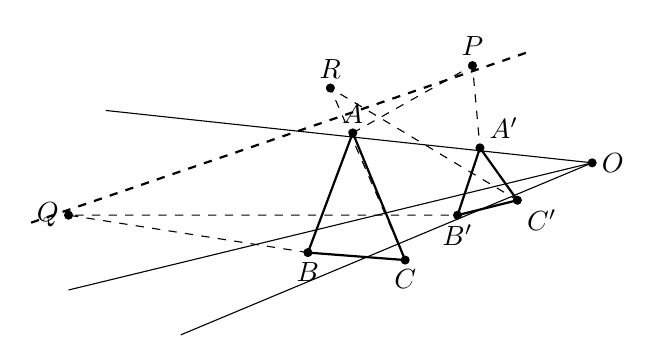
\begin{tikzpicture}[scale=0.95]
  % Center of perspectivity O
  \coordinate (O) at (5.0,0.5);
  \filldraw (O) circle (1.5pt) node[right] {$O$};
  
  % Rays from O
  \coordinate (Aprime) at (3.5,0.7);
  \coordinate (A) at (1.8,0.9);
  \coordinate (Bprime) at (3.2,-0.2);
  \coordinate (B) at (1.2,-0.7);
  \coordinate (Cprime) at (4.0,0.0);
  \coordinate (C) at (2.5,-0.8);
  
  \draw[thin] (O) -- (-1.5,1.2);
  \draw[thin] (O) -- (-2.0,-1.2);
  \draw[thin] (O) -- (-0.5,-1.8);
  
  % Triangles ABC and A'B'C'
  \draw[thick] (A) -- (B) -- (C) -- cycle;
  \draw[thick] (Aprime) -- (Bprime) -- (Cprime) -- cycle;
  
  \filldraw (A) circle (1.5pt) node[above] {$A$};
  \filldraw (B) circle (1.5pt) node[below] {$B$};
  \filldraw (C) circle (1.5pt) node[below] {$C$};
  \filldraw (Aprime) circle (1.5pt) node[above right] {$A'$};
  \filldraw (Bprime) circle (1.5pt) node[below] {$B'$};
  \filldraw (Cprime) circle (1.5pt) node[below right] {$C'$};
  
  % Intersections P, Q, R
  \coordinate (P) at (3.4,1.8);
  \coordinate (R) at (1.5,1.5);
  \coordinate (Q) at (-2.0,-0.2);
  
  \filldraw (P) circle (1.5pt) node[above] {$P$};
  \filldraw (R) circle (1.5pt) node[above] {$R$};
  \filldraw (Q) circle (1.5pt) node[left] {$Q$};
  
  \draw[thick, dashed] (-2.5,-0.3) -- (4.2,2.0);
  \draw[dashed] (A) -- (P) -- (Aprime);
  \draw[dashed] (B) -- (Q) -- (Bprime);
  \draw[dashed] (C) -- (R) -- (Cprime);
\end{tikzpicture}
\caption{笛沙格（Desargues）透視定理}
\label{fig:5-21}
\end{figure}

\begin{proof}[證明]
設 $AA', BB', CC'$ 的交點為 $O$，令向量 $\mathbf{a} = \vec{OA},\; \mathbf{b} = \vec{OB},\; \mathbf{c} = \vec{OC}$，則
\[ \mathbf{a}' = \vec{OA}' = \alpha \mathbf{a},\quad \mathbf{b}' = \vec{OB}' = \beta \mathbf{b},\quad \mathbf{c}' = \vec{OC}' = \gamma \mathbf{c}. \]
設一組對應邊 $AB, A'B'$ 的交點為 $P$，則
\begin{align*}
\vec{OP} &= \lambda \mathbf{a}' + \mu \mathbf{b}' \; (\lambda + \mu = 1) \\
&= \lambda \alpha \mathbf{a} + \mu \beta \mathbf{b},\; (\lambda \alpha + \mu \beta = 1)
\end{align*}
由上式可解出
\[ \lambda = \frac{\beta - 1}{\beta - \alpha},\quad \mu = \frac{\alpha - 1}{\alpha - \beta} \]
因此
\[ \vec{OP} = \frac{\alpha(\beta - 1)}{\beta - \alpha}\mathbf{a} + \frac{\beta(\alpha - 1)}{\alpha - \beta}\mathbf{b} \]
再設 $BC, B'C'$ 之交點為 $Q$；$CA, C'A'$ 之交點為 $R$．
則
\begin{align*}
\vec{OQ} &= \frac{\beta(\gamma - 1)}{\gamma - \beta}\mathbf{b} + \frac{\gamma(\beta - 1)}{\beta - \gamma}\mathbf{c} \\
\vec{OR} &= \frac{\gamma(\alpha - 1)}{\alpha - \gamma}\mathbf{c} + \frac{\alpha(\gamma - 1)}{\gamma - \alpha}\mathbf{a}
\end{align*}
考慮
\begin{align*}
(\gamma - 1)(\beta - \alpha)\vec{OP} &= \alpha(\beta - 1)(\gamma - 1)\mathbf{a} - \beta(\alpha - 1)(\gamma - 1)\mathbf{b} \\
(\alpha - 1)(\gamma - \beta)\vec{OQ} &= \beta(\gamma - 1)(\alpha - 1)\mathbf{b} - \gamma(\beta - 1)(\alpha - 1)\mathbf{c} \\
(\beta - 1)(\alpha - \gamma)\vec{OR} &= \gamma(\alpha - 1)(\beta - 1)\mathbf{c} - \alpha(\gamma - 1)(\beta - 1)\mathbf{a}
\end{align*}
兩端分別相加，得\phantomsection\label{note:b3-ch5-p249-double-minus}\footnote{【原書註記/校訂】：原書第三項係數印作「$+(\beta--1)$」，連印兩個減號，實為「$(\beta - 1)$」，此處予以校訂．}
\[ (\gamma - 1)(\beta - \alpha)\vec{OP} + (\alpha - 1)(\gamma - \beta)\vec{OQ} + (\beta - 1)(\alpha - \gamma)\vec{OR} = \mathbf{0} \]
這個式子就表示 $P, Q, R$ 三點共線．
\end{proof}

\subsubsection*{作業 10}
\begin{enumerate}[label=(\roman*), leftmargin=2.5em]
  \item 證明四邊形對邊中點所聯線段互相平分．
  \item 若（如圖 5-22\phantomsection\label{note:b3-ch5-p249-fig-ref}\footnote{【原書註記/校訂】：原書印作「若（如圖 5-7）」，而本頁下方對應插圖編號實為「圖 5-22」．}）$2\vec{OM} = \vec{OA} + \vec{OB}$，則 $A, M, B$ 三點共線，而且 $M$ 為線段 $AB$ 的中點．
\end{enumerate}

\begin{figure}[H]
\centering
\begin{tikzpicture}[scale=0.95]
  \coordinate (O) at (0,0);
  \coordinate (A) at (3.5,1.8);
  \coordinate (B) at (4.5,0.2);
  \coordinate (M) at ($(A)!0.5!(B)$);
  
  \draw[thick, -{Stealth}] (O) -- (A) node[above right] {$A$};
  \draw[thick, -{Stealth}] (O) -- (B) node[right] {$B$};
  \draw[thick, -{Stealth}] (O) -- (M) node[right] {$M$};
  \draw[thick] (A) -- (B);
  
  \filldraw (O) circle (1.5pt) node[left] {$O$};
  \filldraw (A) circle (1.5pt);
  \filldraw (B) circle (1.5pt);
  \filldraw (M) circle (1.5pt);
\end{tikzpicture}
\caption{線段中點之向量表示}
\label{fig:5-22}
\end{figure}

\subsubsection*{作業 11}
設兩個三角形 $\triangle ABC, \triangle A'B'C'$ 中，對應頂點的 $AA', BB', CC'$ 皆平行，試證三組對應邊的交點共線．

% ==========================================
% § 5-4 幾個利用古典平面幾何處理的極小問題
% ==========================================
\subsection{\texorpdfstring{$\ddagger$ }{‡ }幾個利用古典平面幾何處理的極小問題}\label{sec:b3-5-4}

\subsubsection*{甲、光的反射}

光學上有一個很基本的原理：“在均勻介質中，光沿最短路徑進行．”

設 $L$ 為一反射鏡面，$P$ 為光源，$E$ 為觀察者，欲求光自 $P$ 出發，經在鏡面 $L$ 反射後，進行到觀察者 $E$ 的實際路徑，亦卽欲求 $L$ 反射點 $Q$，使折線 $\{PQ, QE\}$ 正是光從 $P$ 經反射到 $E$ 的路徑．

用數學語言來說明，變成了這樣一個極小問題：“欲在平面（直線）$L$ 上求一點 $Q$，使 $\overline{PQ} + \overline{QE}$ 的距離為最短．”

自 $P$ 引 $L$ 的垂線 $PP_1$ 使交 $L$ 於 $A$，且 $\overline{PA} = \overline{AP_1}$（此時 $P_1$ 稱為 $P$ 在 $L$ 中的鏡像點）設 $Q$ 為 $L$ 上的一般點，則因 $\triangle PQA$ 與 $\triangle P_1QA$ 全等，$\overline{PQ} = \overline{P_1Q}$，故
\[ \overline{PQ} + \overline{QE} = \overline{P_1Q} + \overline{QE} \]
欲使此值為最小，須置 $Q$，使 $P_1, Q, E$ 共線．

換句話說，要求得反射點的辦法是：先取 $P$ 在 $L$ 中的像點 $P_1$，連結 $P_1E$，其與 $L$ 的交點 $Q$ 卽為所求．

\begin{figure}[H]
\centering
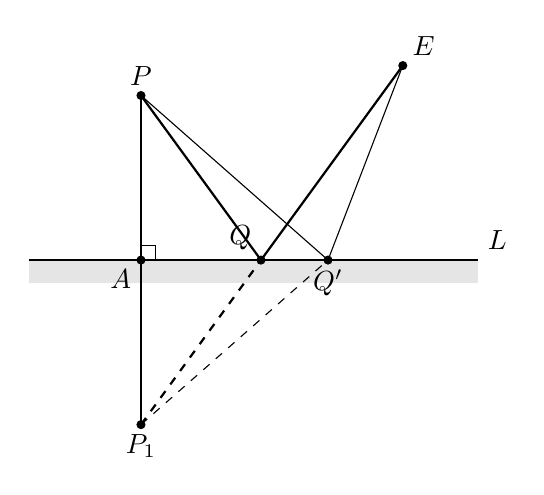
\begin{tikzpicture}[scale=0.95]
  % Mirror L
  \fill[gray!20] (-0.5,-0.3) rectangle (5.5,0);
  \draw[thick] (-0.5,0) -- (5.5,0) node[above right] {$L$};
  
  \coordinate (A) at (1.0,0);
  \coordinate (P) at (1.0,2.2);
  \coordinate (P1) at (1.0,-2.2);
  \coordinate (E) at (4.5,2.6);
  \coordinate (Q) at (intersection of P1--E and A--5.5,0);
  \coordinate (Qprime) at (3.5,0);
  
  \draw[thick] (P) -- (P1);
  \draw[thick] (P) -- (Q) -- (E);
  \draw[thick, dashed] (P1) -- (Q);
  \draw (P) -- (Qprime) -- (E);
  \draw[dashed] (P1) -- (Qprime);
  
  \filldraw (P) circle (1.5pt) node[above] {$P$};
  \filldraw (P1) circle (1.5pt) node[below] {$P_1$};
  \filldraw (E) circle (1.5pt) node[above right] {$E$};
  \filldraw (A) circle (1.5pt) node[below left] {$A$};
  \filldraw (Q) circle (1.5pt) node[above left] {$Q$};
  \filldraw (Qprime) circle (1.5pt) node[below] {$Q'$};
  
  % Right angle mark at A
  \draw (A) rectangle ++(0.2,0.2);
\end{tikzpicture}
\caption{光之反射與鏡像點最短路徑}
\label{fig:5-23}
\end{figure}

由這裏，我們更得到一個光學結果：“入射角與反射角相等”，這是因為：
\[ \angle PQA = \angle P_1QA = \angle EQB \quad \text{〔因 } \triangle PQA \text{ 與 } \triangle P_1QA \text{ 全等〕} \]

\begin{example}[例 7]
有一長形物體 $AB$ 立於地上，朝一垂直立於距 $A$ 10 公尺處 $C$ 點的鏡面傾斜，傾斜角為 $\frac{\pi}{3}$．設 $\overline{AB} = 16$ 公尺．設若在 $A$ 處觀察，鏡面須多高才能在鏡中看到整個物體 $AB$？
\end{example}

\begin{figure}[H]
\centering
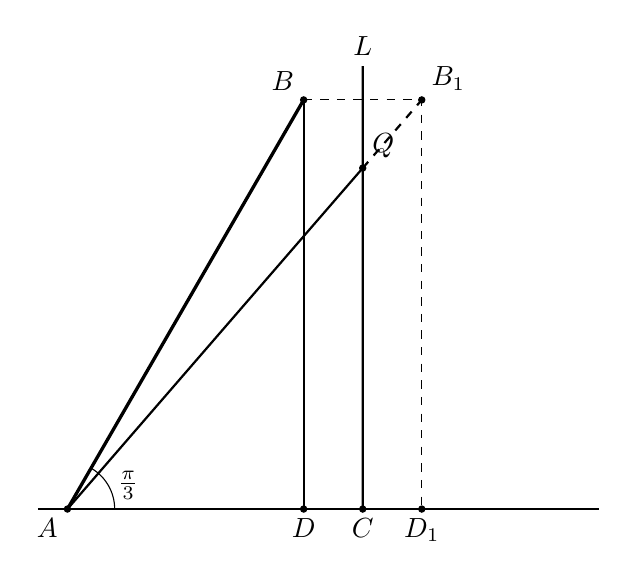
\begin{tikzpicture}[scale=0.75]
  % Ground line
  \draw[thick] (-0.5,0) -- (9.0,0);
  
  \coordinate (A) at (0,0);
  \coordinate (D) at (4.0,0);
  \coordinate (C) at (5.0,0);
  \coordinate (D1) at (6.0,0);
  
  \coordinate (B) at (4.0, 6.928);
  \coordinate (B1) at (6.0, 6.928);
  \coordinate (Q) at (5.0, 5.7735);
  
  % Stick AB
  \draw[very thick] (A) -- (B);
  \draw[thick] (B) -- (D);
  \draw[thick] (C) -- (5.0,7.5) node[above] {$L$};
  
  % Images
  \draw[dashed] (B) -- (B1) -- (D1);
  \draw[thick] (A) -- (Q);
  \draw[thick, dashed] (Q) -- (B1);
  
  \filldraw (A) circle (1.5pt) node[below left] {$A$};
  \filldraw (B) circle (1.5pt) node[above left] {$B$};
  \filldraw (C) circle (1.5pt) node[below] {$C$};
  \filldraw (D) circle (1.5pt) node[below] {$D$};
  \filldraw (D1) circle (1.5pt) node[below] {$D_1$};
  \filldraw (B1) circle (1.5pt) node[above right] {$B_1$};
  \filldraw (Q) circle (1.5pt) node[above right] {$Q$};
  
  % Angle pi/3
  \draw (0.8,0) arc (0:60:0.8) node[midway, right] {$\frac{\pi}{3}$};
\end{tikzpicture}
\caption{傾斜物體鏡中全像視野計算}
\label{fig:5-24}
\end{figure}

\begin{proof}[解]
設 $BD$ 垂直於地面．$B_1, D_1$ 分別為 $B, D$ 在 $L$ 中的像，點 $Q$ 為 $B$ 到 $A$ 的反射點，則
\begin{align*}
\overline{AD} &= \overline{AB} \cos \frac{\pi}{3} = 16 \times \frac{1}{2} = 8 \text{（公尺）} \\
\overline{B_1D_1} &= \overline{BD} = \overline{AB} \sin \frac{\pi}{3} = 16 \times \frac{\sqrt{3}}{2} = 8\sqrt{3} \text{（公尺）} \\
\overline{AD_1} &= \overline{AC} + \overline{CD_1} = 10 + \overline{CD} = 10 + (10 - 8) = 12 \text{（公尺）}
\end{align*}
而
\[ \frac{\overline{QC}}{\overline{B_1D_1}} = \frac{\overline{AC}}{\overline{AD_1}} = \frac{10}{12} = \frac{5}{6}, \]
故 $\overline{QC} = \frac{5}{6} \cdot 8\sqrt{3} = \frac{20}{3}\sqrt{3} = \frac{20}{\sqrt{3}}$ \\
卽鏡面至少須 $\frac{20}{\sqrt{3}}$ 公尺才能自 $A$ 在鏡中看到整個 $AB$．
\end{proof}

\subsubsection*{乙、到三定點的最小距離和\phantomsection\label{note:b3-ch5-p251-sec-title}\footnote{【原書註記/校訂】：原書小節標籤誤印為「八、到三定點的最小距離和」，依大綱順序「甲、光的反射」、「丙、連結三角形三邊的最短路徑」，此處實為「乙」，正文予以保留原標題樣貌並加註．}}

\begin{example}[論例 7]
有三個城鎮 $A, B, C$．今要設一倉庫 $S$，每天由這倉庫向各城鎮輸送補給品，假定一趟只能去一個城鎮，倉庫應設在何處最省運輸費？
\end{example}

這樣的問題化成數學語言便是“給定三點 $A, B, C$，求一點 $S$，使
\[ \overline{AS} + \overline{BS} + \overline{CS} \text{ 為最小？} ” \]

與上節光的反射屬於同一類型，要解決這種問題，通常應朝變成「兩點間距以直線為最短」的方向一步步簡化．像光的反射，原是要求得 $Q$，使 $P$ 經 $Q$ 到 $E$ 為最短路徑，但代以考慮 $P$ 的像點 $P_1$，則問題變成求一路徑連結 $P_1$ 與 $E$，此時自然以直線為最短，接著推回原來的問題得到結果．

這節的運輸問題也是這樣：如果把 $\triangle ASB$ 以 $B$ 為心，往背著 $C$ 的方向，旋轉 $\frac{\pi}{3} = 60^\circ$，得 $\triangle C'TB$ 則 $\overline{AS} = \overline{C'T}$，且 $\triangle SBT$ 中，
\[ \angle SBT = \frac{\pi}{3},\quad \overline{BS} = \overline{BT} \]
頂角為 $60^\circ$ 之等腰三角形必為正三角形．故 $\triangle SBT$ 為正三角形．故
\[ \overline{BS} = \overline{TS} \]
故
\[ \overline{AS} + \overline{BS} + \overline{CS} = \overline{C'T} + \overline{TS} + \overline{SC} \]
因此，當 $S$ 與 $T$ 皆在 $\overline{CC'}$ 線上時，$\overline{AS} + \overline{BS} + \overline{CS}$ 為最小．

這樣的可能是唯一的．因 $CC'$ 上只有唯一的一對點 $S$ 與 $T$，會使得 $\triangle BST$ 成為正三角形．故欲求 $S$，只須過 $B$ 作 $BS$，使
\[ \angle BSC' = \frac{\pi}{3} = 60^\circ \]
即可．

\begin{figure}[H]
\centering
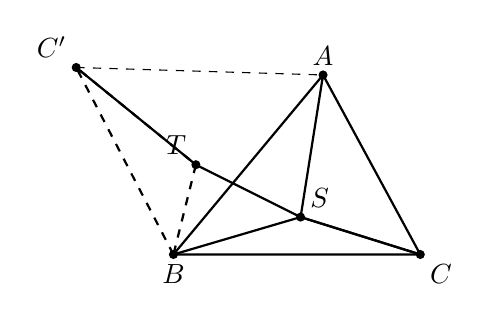
\begin{tikzpicture}[scale=0.95]
  \coordinate (B) at (1.5,0.8);
  \coordinate (A) at (3.5,3.2);
  \coordinate (C) at (4.8,0.8);
  
  \coordinate (Cprime) at (0.2,3.3);
  \coordinate (T) at (1.8,2.0);
  \coordinate (S) at (3.2,1.3);
  
  \draw[thick] (A) -- (B) -- (C) -- cycle;
  \draw[thick] (A) -- (S);
  \draw[thick] (B) -- (S);
  \draw[thick] (C) -- (S);
  
  \draw[thick, dashed] (B) -- (Cprime) -- (T) -- cycle;
  \draw[thick] (Cprime) -- (T) -- (S) -- (C);
  \draw[dashed] (Cprime) -- (A);
  
  \filldraw (A) circle (1.5pt) node[above] {$A$};
  \filldraw (B) circle (1.5pt) node[below] {$B$};
  \filldraw (C) circle (1.5pt) node[below right] {$C$};
  \filldraw (Cprime) circle (1.5pt) node[above left] {$C'$};
  \filldraw (T) circle (1.5pt) node[above left] {$T$};
  \filldraw (S) circle (1.5pt) node[above right] {$S$};
\end{tikzpicture}
\caption{旋轉 $60^\circ$ 化簡之費馬點問題}
\label{fig:5-25}
\end{figure}

很自然地，既然滿足 $\overline{AS} + \overline{BS} + \overline{CS}$ 為最小的點 $S$ 是已知存在而且唯一．而它要落在 $CC'$ 線上，那麼，若我們類推地作出 $B', A'$ 點（如圖）．則 $S$ 也應該落在 $BB'$ 上，落在 $AA'$ 上．

其實，我們也附帶證明了 $AA', BB', CC'$ 三線交於一點，而這點便是我們所求的 $S$ 點．它到 $A, B, C$ 三定點的和正好是 $\overline{CC'} (= \overline{BB'} = \overline{AA'})$．

以下事實的檢驗，可以幫助我們的了解：「若取 $S$ 為 $CC'$ 與 $BB'$ 交點，則 $\angle BSC' = \frac{\pi}{3}$．」這是因為 $\triangle ABB'$ 與 $\triangle AC'C$ 全等，故 $\angle ABB' = \angle AC'C$，故設 $D$ 為 $CC'$ 與 $AB$ 邊交點，則
\begin{align*}
\angle BSC' &= \pi - (\angle ABB' + \angle BDS) = \pi - (\angle AC'C + \angle C'DA) \\
&= \angle BAC' = \frac{\pi}{3}.
\end{align*}
因此知道，正是 $CC'$ 與 $BB'$ 的交點，向 $B$ 與 $C'$ 張著 $\frac{\pi}{3}$ 的角．同理也向著 $B'C$ 張著 $\frac{\pi}{3}$ 的角．

我們更得到：
\begin{center}
\parbox{0.92\textwidth}{「滿足 $\overline{AS} + \overline{BS} + \overline{CS}$ 為最小的點 $S$，向三定點 $A, B, C$ 分別張著 $\frac{2\pi}{3}$ 的角，卽 $\angle ASB = \angle BSC = \angle CSA = \frac{2\pi}{3}$．」}
\end{center}

\noindent\textbf{結論}\quad 到三定點 $A, B, C$ 之距離和為最小之點 $S$，可依下法尋得：\\
在 $AB, BC, CA$ 各邊分別向外作正三角形 $\triangle ABC', \triangle BCA', \triangle CAB'$，連結 $CC', BB', AA'$ 三線必交於一點，此交點便是所求 $S$，且 $\overline{AS} + \overline{BS} + \overline{CS} = \overline{CC'} = \overline{BB'} = \overline{AA'}$．

\begin{figure}[H]
\centering
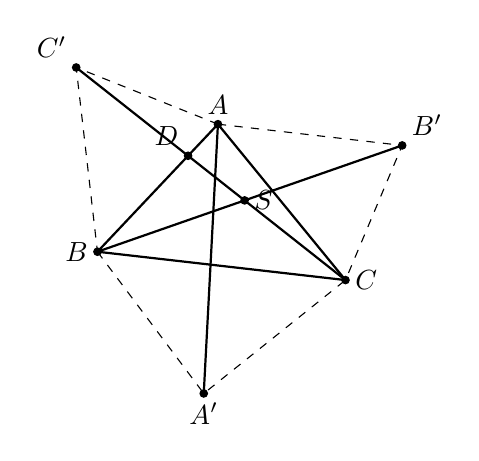
\begin{tikzpicture}[scale=0.9]
  \coordinate (A) at (2.2,3.0);
  \coordinate (B) at (0.5,1.2);
  \coordinate (C) at (4.0,0.8);
  
  \draw[thick] (A) -- (B) -- (C) -- cycle;
  
  % External equilateral triangles
  \coordinate (Cprime) at (0.2,3.8);
  \coordinate (Aprime) at (2.0,-0.8);
  \coordinate (Bprime) at (4.8,2.7);
  
  \draw[dashed] (A) -- (Cprime) -- (B);
  \draw[dashed] (B) -- (Aprime) -- (C);
  \draw[dashed] (A) -- (Bprime) -- (C);
  
  % Concurrency lines
  \draw[thick] (C) -- (Cprime);
  \draw[thick] (B) -- (Bprime);
  \draw[thick] (A) -- (Aprime);
  
  % Intersection S
  \coordinate (S) at (intersection of C--Cprime and B--Bprime);
  \filldraw (S) circle (1.5pt) node[right] {$S$};
  
  \filldraw (A) circle (1.5pt) node[above] {$A$};
  \filldraw (B) circle (1.5pt) node[left] {$B$};
  \filldraw (C) circle (1.5pt) node[right] {$C$};
  \filldraw (Cprime) circle (1.5pt) node[above left] {$C'$};
  \filldraw (Aprime) circle (1.5pt) node[below] {$A'$};
  \filldraw (Bprime) circle (1.5pt) node[above right] {$B'$};
  
  \coordinate (D) at (intersection of C--Cprime and A--B);
  \filldraw (D) circle (1.5pt) node[above left] {$D$};
\end{tikzpicture}
\caption{三角形三外側正三角形頂點連線交於費馬點}
\label{fig:5-26}
\end{figure}

\subsubsection*{* 丙、連結三角形三邊的最短路徑}

\begin{example}[論例 8]
在 $\triangle ABC$ 三邊上求三點 $A', B', C'$，使 $\overline{A'B'} + \overline{B'C'} + \overline{C'A'}$ 為最小．
\end{example}

\noindent\underline{第一步}\quad 先考慮一個較單純的問題：
\begin{center}
\parbox{0.92\textwidth}{「設已取定 $BC$ 邊長的一點 $A'$，求 $AC, AB$ 邊上兩點 $B', C'$，使 $\overline{A'B'} + \overline{B'C'} + \overline{C'A'}$ 為最小．」}
\end{center}

\begin{figure}[H]
\centering
\begin{subfigure}[b]{0.45\textwidth}
  \centering
  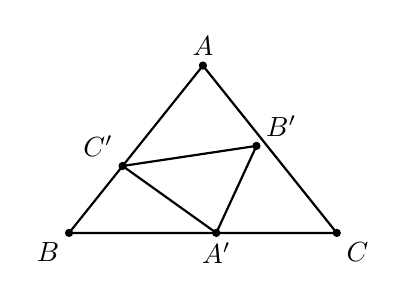
\begin{tikzpicture}[scale=0.85]
    \coordinate (A) at (2.0,3.0);
    \coordinate (B) at (0,0.5);
    \coordinate (C) at (4.0,0.5);
    \coordinate (Aprime) at (2.2,0.5);
    \coordinate (Bprime) at (2.8,1.8);
    \coordinate (Cprime) at (0.8,1.5);
    
    \draw[thick] (A) -- (B) -- (C) -- cycle;
    \draw[thick] (Aprime) -- (Bprime) -- (Cprime) -- cycle;
    
    \filldraw (A) circle (1.5pt) node[above] {$A$};
    \filldraw (B) circle (1.5pt) node[below left] {$B$};
    \filldraw (C) circle (1.5pt) node[below right] {$C$};
    \filldraw (Aprime) circle (1.5pt) node[below] {$A'$};
    \filldraw (Bprime) circle (1.5pt) node[above right] {$B'$};
    \filldraw (Cprime) circle (1.5pt) node[above left] {$C'$};
  \end{tikzpicture}
  \caption{三角形之內接三角形}
  \label{fig:5-27}
\end{subfigure}
\hfill
\begin{subfigure}[b]{0.48\textwidth}
  \centering
  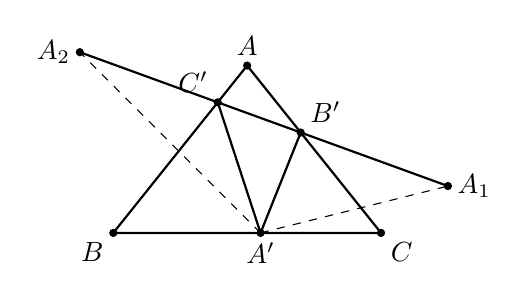
\begin{tikzpicture}[scale=0.85]
    \coordinate (A) at (2.0,3.0);
    \coordinate (B) at (0,0.5);
    \coordinate (C) at (4.0,0.5);
    \coordinate (Aprime) at (2.2,0.5);
    
    % Reflections of A' across AC and AB
    \coordinate (A1) at (5.0,1.2);
    \coordinate (A2) at (-0.5,3.2);
    
    \draw[thick] (A) -- (B) -- (C) -- cycle;
    \draw[thick] (A1) -- (A2);
    
    \coordinate (Bprime) at (intersection of A1--A2 and A--C);
    \coordinate (Cprime) at (intersection of A1--A2 and A--B);
    
    \draw[thick] (Aprime) -- (Bprime);
    \draw[thick] (Aprime) -- (Cprime);
    \draw[dashed] (Aprime) -- (A1);
    \draw[dashed] (Aprime) -- (A2);
    
    \filldraw (A) circle (1.5pt) node[above] {$A$};
    \filldraw (B) circle (1.5pt) node[below left] {$B$};
    \filldraw (C) circle (1.5pt) node[below right] {$C$};
    \filldraw (Aprime) circle (1.5pt) node[below] {$A'$};
    \filldraw (A1) circle (1.5pt) node[right] {$A_1$};
    \filldraw (A2) circle (1.5pt) node[left] {$A_2$};
    \filldraw (Bprime) circle (1.5pt) node[above right] {$B'$};
    \filldraw (Cprime) circle (1.5pt) node[above left] {$C'$};
  \end{tikzpicture}
  \caption{鏡像展開為直線段化簡法尼亞諾問題}
  \label{fig:5-28}
\end{subfigure}
\end{figure}

再一次，我們要把它簡化成「兩點間距直線最短」的型式．取 $A'$ 分別對於 $AC, AB$ 的鏡像點 $A_1, A_2$．連結 $A_1A_2$ 交 $AC, AB$ 邊於 $B', C'$．則
\[ \overline{A'B'} + \overline{B'C'} + \overline{C'A'} \]
在 $A'$ 固定時為最短路徑，因若有其他在 $AC, AB$ 邊上的兩點 $B'', C''$，則
\begin{align*}
\overline{A'B''} + \overline{B''C''} + \overline{C''A'} &= \overline{A_1B''} + \overline{B''C''} + \overline{C''A_2} \\
&\ge \overline{A_1A_2} = \overline{A_1B'} + \overline{B'C'} + \overline{C'A_2} = \overline{A'B'} + \overline{B'C'} + \overline{C'A'}
\end{align*}

\noindent\underline{第二步} \\
我們注意到第一步中之 $\triangle A_1AA_2$ 之頂角 $\angle A_1AA_2 = 2\angle BAC$．（此因 $\angle A'AC = \angle A_1AC$，且 $\angle A'AB = \angle A_2AB$ 之故．）而且
\[ \overline{AA_1} = \overline{AA'} = \overline{AA_2} \]
因此不拘一開始 $A'$ 固定在 $BC$ 邊上那個位置，所相應的 $\triangle A_1AA_2$ 是一個頂角之大小已固定為 $2\angle BAC$ 的一個等腰三角形，其腰長越小，底邊也越小．

但其腰 $\overline{AA_1} = \overline{AA'}$，故當 $\overline{AA'}$ 為最小時，$\overline{A_1A_2}$ 為最小亦卽
\[ \overline{A'B'} + \overline{B'C'} + \overline{C'A'} \text{ 為最小．} \]
可是由定點 $A$ 到 $BC$ 邊上的 $A'$ 點之距離 $\overline{AA'}$，在 $\overline{AA'}$ 垂直於 $BC$ 邊時為最小，換句話說：所求的 $A'$ 點為 $A$ 向 $BC$ 所引垂線的垂足．同理 $B', C'$ 亦分別為自 $B, C$ 向 $CA, AB$ 所引直線的垂足．而此時 $\overline{A'B'} + \overline{B'C'} + \overline{C'A'}$ 為最小，且其值等於 $\overline{A_1A_2}$，其中 $A_1, A_2$ 分別為 $A'$ 對於 $CA, BC$\phantomsection\label{note:b3-ch5-p255-mirror-line}\footnote{【原書註記/校訂】：原書印作「對於 $CA, BC$ 的鏡像點」，依前文推導明確為對 $AC$ 與 $AB$ 邊之鏡像點．正文保留原字樣並加註．} 的鏡像點．

\begin{figure}[H]
\centering
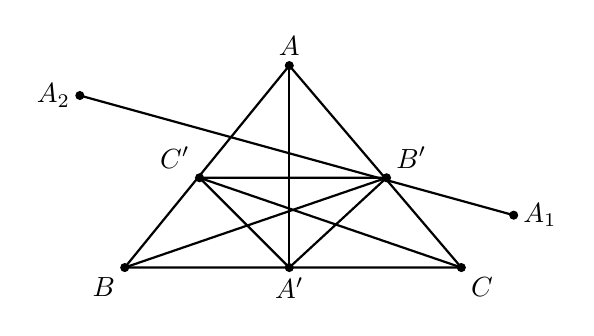
\begin{tikzpicture}[scale=0.95]
  \coordinate (A) at (2.2,3.2);
  \coordinate (B) at (0,0.5);
  \coordinate (C) at (4.5,0.5);
  
  \coordinate (Aprime) at (2.2,0.5);
  \coordinate (Bprime) at (3.5,1.7);
  \coordinate (Cprime) at (1.0,1.7);
  
  \coordinate (A1) at (5.2,1.2);
  \coordinate (A2) at (-0.6,2.8);
  
  \draw[thick] (A) -- (B) -- (C) -- cycle;
  \draw[thick] (A) -- (Aprime);
  \draw[thick] (B) -- (Bprime);
  \draw[thick] (C) -- (Cprime);
  
  \draw[thick] (Aprime) -- (Bprime) -- (Cprime) -- cycle;
  \draw[thick] (A1) -- (A2);
  
  \filldraw (A) circle (1.5pt) node[above] {$A$};
  \filldraw (B) circle (1.5pt) node[below left] {$B$};
  \filldraw (C) circle (1.5pt) node[below right] {$C$};
  \filldraw (Aprime) circle (1.5pt) node[below] {$A'$};
  \filldraw (Bprime) circle (1.5pt) node[above right] {$B'$};
  \filldraw (Cprime) circle (1.5pt) node[above left] {$C'$};
  \filldraw (A1) circle (1.5pt) node[right] {$A_1$};
  \filldraw (A2) circle (1.5pt) node[left] {$A_2$};
\end{tikzpicture}
\caption{垂足三角形（Orthic triangle）與最短周長}
\label{fig:5-29}
\end{figure}

\noindent\underline{第三步} \\
我們算一下 $\overline{A_1A_2}$，根據餘弦定律
\[ \overline{A_1A_2}^2 = 2\alpha^2 - 2\alpha^2 \cos 2A = 2\alpha^2(1 - \cos 2A) \]
其中 $\alpha = \overline{AA_2} = \overline{AA_1} = \overline{AA'},\quad A = \triangle ABC \text{ 的頂角 } \angle BAC \text{ 角度}$ \\
由習題中，知 $(1 - \cos 2A) = 2\sin^2 A$ \\
故 $\overline{A_1A_2} = 2\alpha \sin A$

總結一下，我們有

\begin{theorem*}[結論]
連結 $\triangle ABC$ 三邊的最短路徑為由三條垂線之垂足 $A', B', C'$ 所構成的三角路徑，且這路徑的長為
\[ 2h_1 \sin A = 2h_2 \sin B = 2h_3 \sin C \]
其中 $h_1, h_2, h_3$ 分別為垂線長 $\overline{AA'}, \overline{BB'}, \overline{CC'}$．
\end{theorem*}

\begin{example}[論例 9]
設有四個村莊處於邊長為 10 公里之正方形的四個頂點上，今要築一鄉道，將這四個村莊連在一起，問何種路線為最經濟？並計算此路線之長度．
\end{example}

\noindent\textbf{註：}本論例可應用在十字路口人行地道的挖築．

\begin{proof}[解]
首先，我們可以證明最經濟的路線中所有的叉路都是三叉路，而且所有的三叉路的夾角都是 $\frac{2\pi}{3}$．譬如說，在路線中，假如有一個叉路口，其中有一個夾角小於 $\frac{2\pi}{3}$（卽 $\angle POQ < \frac{2\pi}{3}$），則我們可以把 $\{OP \cup OQ\}$ 這一段路線改成較短的路線 $\{OF \cup FP \cup FQ\}$，其中 $OF, FP, FQ$ 的夾角都是 $\frac{2\pi}{3}$，所以當路線是最短可能時，其叉路口的每一夾角都得 $\ge \frac{2\pi}{3}$，但是一個叉路口至少有三個夾角，其角度的總和是 $2\pi$，所以只能有三叉路口，而且其每一夾角正好是 $\frac{2\pi}{3}$．

\begin{figure}[H]
\centering
\begin{subfigure}[b]{0.48\textwidth}
  \centering
  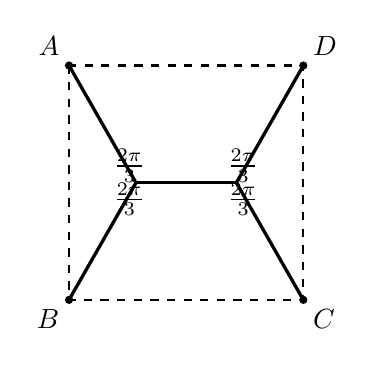
\begin{tikzpicture}[scale=0.85]
    % Square ABCD
    \coordinate (A) at (0,3.5);
    \coordinate (B) at (0,0);
    \coordinate (C) at (3.5,0);
    \coordinate (D) at (3.5,3.5);
    
    \draw[thick, dashed] (A) -- (B) -- (C) -- (D) -- cycle;
    
    \coordinate (P) at (1.0, 1.75);
    \coordinate (Q) at (2.5, 1.75);
    
    \draw[very thick] (A) -- (P);
    \draw[very thick] (B) -- (P);
    \draw[very thick] (P) -- (Q);
    \draw[very thick] (D) -- (Q);
    \draw[very thick] (C) -- (Q);
    
    \filldraw (A) circle (1.5pt) node[above left] {$A$};
    \filldraw (B) circle (1.5pt) node[below left] {$B$};
    \filldraw (C) circle (1.5pt) node[below right] {$C$};
    \filldraw (D) circle (1.5pt) node[above right] {$D$};
    
    \node at (0.9,2.0) {$\frac{2\pi}{3}$};
    \node at (0.9,1.5) {$\frac{2\pi}{3}$};
    \node at (2.6,2.0) {$\frac{2\pi}{3}$};
    \node at (2.6,1.5) {$\frac{2\pi}{3}$};
  \end{tikzpicture}
  \caption{正方形四頂點之斯坦納最小樹}
  \label{fig:5-30}
\end{subfigure}
\hfill
\begin{subfigure}[b]{0.45\textwidth}
  \centering
  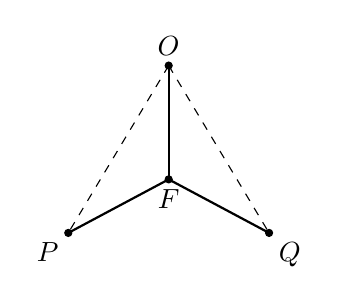
\begin{tikzpicture}[scale=0.85]
    \coordinate (O) at (1.5,2.5);
    \coordinate (P) at (0,0);
    \coordinate (Q) at (3.0,0);
    \coordinate (F) at (1.5,0.8);
    
    \draw[thick] (O) -- (F);
    \draw[thick] (P) -- (F);
    \draw[thick] (Q) -- (F);
    \draw[dashed] (O) -- (P);
    \draw[dashed] (O) -- (Q);
    
    \filldraw (O) circle (1.5pt) node[above] {$O$};
    \filldraw (P) circle (1.5pt) node[below left] {$P$};
    \filldraw (Q) circle (1.5pt) node[below right] {$Q$};
    \filldraw (F) circle (1.5pt) node[below] {$F$};
  \end{tikzpicture}
  \caption{三叉路夾角 $120^\circ$ 之局部變分優化}
  \label{fig:5-31}
\end{subfigure}
\end{figure}

假設圖 5-32 所示 $P, Q$ 的三叉路是一種最短的路線，$P, Q$ 是它的二個三叉路口，則由上面的討論，知道在 $P, Q$ 的分叉角都是 $\frac{2\pi}{3}$，所以由內角和定理，有下述關係：
\begin{align*}
\angle 1 + \angle 2 &= \angle 3 + \angle 4 = \frac{\pi}{3} \\
\angle 1' + \angle 4' &= \angle 2' + \angle 3' = \left( 2\pi - \frac{4\pi}{3} \right) = \frac{2\pi}{3} \\
\text{亦卽}\quad \left( \frac{\pi}{2} - \angle 1 \right) + \left( \frac{\pi}{2} - \angle 4 \right) &= \left( \frac{\pi}{2} - \angle 2 \right) + \left( \frac{\pi}{2} - \angle 3 \right) = \frac{2\pi}{3}
\end{align*}

\begin{figure}[H]
\centering
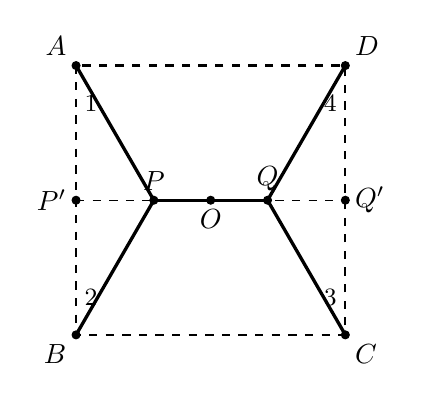
\begin{tikzpicture}[scale=0.95]
  % Square ABCD
  \coordinate (A) at (0,3.6);
  \coordinate (B) at (0,0);
  \coordinate (C) at (3.6,0);
  \coordinate (D) at (3.6,3.6);
  
  \draw[thick, dashed] (A) -- (B) -- (C) -- (D) -- cycle;
  
  \coordinate (P) at (1.04, 1.8);
  \coordinate (Q) at (2.56, 1.8);
  \coordinate (O) at (1.8, 1.8);
  
  \coordinate (Pprime) at (0, 1.8);
  \coordinate (Qprime) at (3.6, 1.8);
  
  \draw[very thick] (A) -- (P);
  \draw[very thick] (B) -- (P);
  \draw[very thick] (P) -- (Q);
  \draw[very thick] (D) -- (Q);
  \draw[very thick] (C) -- (Q);
  
  \draw[thin, dashed] (Pprime) -- (Qprime);
  
  \filldraw (A) circle (1.5pt) node[above left] {$A$};
  \filldraw (B) circle (1.5pt) node[below left] {$B$};
  \filldraw (C) circle (1.5pt) node[below right] {$C$};
  \filldraw (D) circle (1.5pt) node[above right] {$D$};
  \filldraw (P) circle (1.5pt) node[above] {$P$};
  \filldraw (Q) circle (1.5pt) node[above] {$Q$};
  \filldraw (O) circle (1.5pt) node[below] {$O$};
  \filldraw (Pprime) circle (1.5pt) node[left] {$P'$};
  \filldraw (Qprime) circle (1.5pt) node[right] {$Q'$};
  
  % Angle labels
  \node at (0.2,3.1) {\small 1};
  \node at (0.2,0.5) {\small 2};
  \node at (3.4,0.5) {\small 3};
  \node at (3.4,3.1) {\small 4};
\end{tikzpicture}
\caption{正方形斯坦納樹角度與線段長度對稱分析}
\label{fig:5-32}
\end{figure}

故有
\[ \begin{cases} \angle 1 + \angle 4 = \angle 3 + \angle 2 = \frac{\pi}{3} \\ \angle 1 - \angle 4 = \angle 3 - \angle 2 \end{cases} \implies \begin{cases} \angle 1 = \angle 3 \\ \angle 4 = \angle 2 \end{cases} \]
所以可知 $\triangle ABP \cong \triangle CDQ$，而且對於正方形的中心 $O$ 是對稱的，所以 $PQ$ 的中點就是 $O$，由此不難看出
\[ \angle 1 = \angle 2 = \angle 3 = \angle 4 = \frac{\pi}{6}. \]
且可計算路線的總長如下：
\begin{align*}
\overline{AP} &= \overline{BP} = \overline{CQ} = \overline{DQ} = \frac{10}{\sqrt{3}} \text{ 公里} \\
\overline{P'P} &= \overline{QQ'} = \frac{1}{2}\overline{AP} \\
\overline{P'P} + \overline{PQ} + \overline{QQ'} &= 10 \text{ 公里} \\
\text{故有}\quad \overline{AP} + \overline{BP} + \overline{CQ} + \overline{DQ} + \overline{PQ} &= 3\overline{AP} + \{\overline{P'P} + \overline{PQ} + \overline{QQ'}\} \\
&= \left( 3\frac{10}{\sqrt{3}} + 10 \right) \text{公里} \\
&= 10(\sqrt{3} + 1) \text{ 公里}\quad (\text{約 } 27.3 \text{ 公里})
\end{align*}
\end{proof}

\subsubsection*{習題 5-4}
\begin{enumerate}[leftmargin=2em]
  \item $A, B$ 為在直線 $CD$ 兩側之二點，在 $CD$ 上找一個點 $P$，使得 $|\overline{AP} - \overline{BP}|$ 為最大．
  \item 底邊相同，面積一樣大的三角形之中，試證等腰三角形的周界最短．
  \item 底邊相同，周界相等的三角形之中，試證等腰三角形的面積最大．
  \item 如圖 5-33，在所有共用內角 $\angle BAC$，而且其對應邊通過已知點 $P$（在此 $P$ 在 $\angle BAC$ 的內側）的三角形當中，試求出面積最小的三角形．
  \begin{figure}[H]
  \centering
  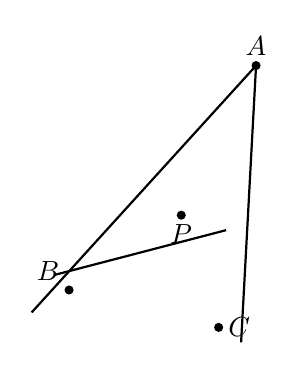
\begin{tikzpicture}[scale=0.95]
    \coordinate (A) at (2.5,3.0);
    \coordinate (B) at (0,0);
    \coordinate (C) at (2.0,-0.5);
    
    \draw[thick] (-0.5,-0.3) -- (A) -- (2.3,-0.7);
    \coordinate (P) at (1.5,1.0);
    
    % Transversal line
    \draw[thick] (-0.2,0.2) -- (2.1,0.8);
    
    \filldraw (A) circle (1.5pt) node[above] {$A$};
    \filldraw (P) circle (1.5pt) node[below] {$P$};
    \filldraw (B) circle (1.5pt) node[above left] {$B$};
    \filldraw (C) circle (1.5pt) node[right] {$C$};
  \end{tikzpicture}
  \caption{角內定點之割線所截三角形面積極小問題}
  \label{fig:5-33}
  \end{figure}

  \item 在已知的正方形的內接正方形之中（如圖 5-34），試求面積為最大的內接正方形．
  \begin{figure}[H]
  \centering
  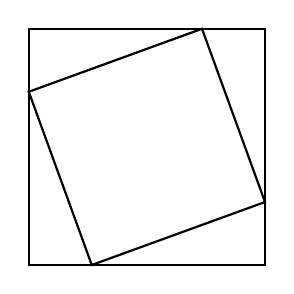
\begin{tikzpicture}[scale=1.0]
    \draw[thick] (0,0) rectangle (3.0,3.0);
    \coordinate (P1) at (0.8,0);
    \coordinate (P2) at (3.0,0.8);
    \coordinate (P3) at (2.2,3.0);
    \coordinate (P4) at (0,2.2);
    
    \draw[thick] (P1) -- (P2) -- (P3) -- (P4) -- cycle;
  \end{tikzpicture}
  \caption{正方形之內接正方形}
  \label{fig:5-34}
  \end{figure}
\end{enumerate}
